% !Mode:: "TeX:UTF-8"
\documentclass[14pt, twoside]{extreport}
\usepackage{cmap}

%\usepackage{fix-cm}
\usepackage[utf8]{inputenx}
\usepackage[russian]{babel}
%%%%%%%%%%%%%%%%%%%%%%%%%%%%\usepackage{pscyr}
%\usepackage[T1]{fontenc} %cm-super
%\usepackage{type1cm}
\usepackage{indentfirst}
\usepackage{amsthm}
\usepackage{amssymb}
\usepackage{amsmath}
%\usepackage{dsfont}
\usepackage{xspace}
\usepackage[numbers,compress,sort]{natbib}
\usepackage{clrscode}

\pagestyle{headings}

\textheight 23cm % 29.7-2-2
\textwidth 16cm % 21-2.5-1.5
\hoffset 0.46cm %2.5-2.54 слева 3 см
\voffset -0.54cm %2-2.54 сверху 2 см
\oddsidemargin 0cm \evensidemargin 0cm  \headheight 0cm \headsep 1.5cm \topmargin 0cm

\usepackage{ccaption} % заменяем для рисунков ':' после номера рисунка на другой символ
\captiondelim{. } % разделитель точка и пробел

\usepackage[off]{auto-pst-pdf}

\usepackage{ifpdf}

\usepackage{vaucanson-g}

\ifpdf
% we are running pdflatex, so convert .eps files to .pdf
% run pdflatex with --shell-escape and thesis.aux
%\usepackage[pdftex]{graphicx}
\usepackage{epstopdf}
\else
% we are running LaTeX, not pdflatex
\usepackage{graphicx}
\fi

% Подправим команду \appendix : нумерация русскими буквами,
% а не латинскими.
\makeatletter
\renewcommand\appendix{\par
  \setcounter{chapter}{0}%
  \setcounter{section}{0}%
  \def\@chapapp{\appendixname}%
  \def\thechapter{\@Asbuk\c@chapter}}
\makeatother

% "русифицируем" окружение enumerate:
\makeatletter
\def\labelenumi{\theenumi)}      % чтобы после номера шла скобка;
\def\theenumii{\@asbuk\c@enumii}   % чтобы на втором уровне шли русские,
\def\labelenumii{\theenumii)}    % а не латинские буквы
\def\p@enumii{\theenumi}         % а это для \ref
\def\labelenumiii{{\bf--}}       % а на третьем уровне пусть будут лишь тире,
\let\theenumiii\relax            % и отдельных ссылок на него не будет
\def\p@enumiii{\theenumi\theenumii}
\makeatother

\usepackage{rsl}

\usepackage{listingsutf8}
\lstloadlanguages{RSL}
\lstset{numbers=left, language=RSL, extendedchars=true, numberstyle=\tiny, inputencoding=utf8%,
%commentstyle=\itshape, stringstyle=\bfseries
}

\author{Евгений Корныхин}
\title{\huge{\textbf{\textsc{Формальная спецификация функциональных свойств конечноавтоматных моделей программ}}}}
%\date{Москва --- 2010}

\newcounter{problem_type}[chapter]
\newcounter{zadacha}[problem_type]
\newcommand{\z}{\vspace{0.5cm}\par\addtocounter{zadacha}{1}%
\textit{\arabic{chapter}.\arabic{problem_type}.\arabic{zadacha}}~~  }

%\newcounter{problem_type}[section]
%\newcounter{zadacha}[problem_type]
%\newcommand{\z}{\vspace{0.5cm}\par\addtocounter{zadacha}{1}%
%\textit{\arabic{section}.\arabic{problem_type}.\arabic{zadacha}}~~  }

\newcommand{\head}[1]{\vspace{1cm}\subsubsection*{#1}}
\newcommand{\zhead}[1]{\head{#1} \refstepcounter{problem_type}}


\begin{document}

\maketitle

\tableofcontents \pagebreak

\section{��������}

��������������� �������� ����� �� ������ ������ ��������������
������. ������� ������������ ����������������, � ��� ����� � ��
��������� ������, �������� ���������� �������. ���������
�������������� ������������ ����������� � �������������� ��������
����� �������� �� ����� ���������� (�������� ��������). �����
��������� ����������� � ������ ������, �����������, ������� ��
���������� ��������������� � ����� �������������. � ����������
��������� �������, � ����� ������� �������������� ���� �����
����������� (������������ ��������� ���������, �������� �� ����, ���
�������� � ������������). ������ ��� ���������� ����������
������������ ��� ����������� ���������������� ��������� ���������
�������� ��������, ��� ������ ���������� ������ ��������������
��������� �������� ��������.

� ������~\cite{kamkin} ���������� ��������������� ������� ����������
�������� �������� �� ������ ������ ���������������. � ������ ����
������� ������� �������� ��������� �������������� �������� �
����������� ���� (� ���� ��������� �������) �- ��� ����������
���������� ����������. �������� ������� ��������� ������������������
����������, ��������� ���������� � ��������� ������������ �������
(��������, ������������, ������� ��� ��������� � ���-������). �
�������� ���������� ���������� ����� ���� ������� �������� �
���������. ������������������ ���������� ���� ����� ������ ����.
������������� � �������� ������� ������ ��������� �����, �����
������������ ���������� ���������� ������� � ��� ���� ��������
������������������� ����������, ������ �� ������� ������ ����
��������� �������� �������.

����� �������� �������� ��������� �� ��������� ��������� �������,
���������� ����� ��������� �������� ��������� � ��� ����� ���-������
� ������ ���������, � �������� �������� ���������� �������.
����������� � ������� ������ ���������� ��������� �������, � ������
�� ���������� � ������� ��������� �������� ������. �� ��������
������ �������� ����� ���������� ������������� ���������������
(�������� �������� � ��������, ��� � �.�.), ������� ����������� �
������ ��������� �������. ���������� ����� ������� ��������
��������� ����� ��������� � ���������, ��������� �� ��������� ������
���������� � ���, ��� ���� �������� � �������� �������. ��� �������
�������� �������� (������� �����������, ������� ������������������
����������) ������ ��������� �������� ������ ���������� ���������
���������, ������� � ��������� ������ ������.



%%%%%%%%%% Общая структура %%%%%%%%%%%
%%  0. "Введение". (см. igoogle) Создание формальной модели поведения системы как способ уточнения требований
%%  1. "Основные определения" (спецификация, модель, полнота, тотальность, непротиворечивость, явность).
%%      Нулевая задачка экзамена. Детерминированные функции, недетерминированные функции на примерах чисел.
%%      Первая задачка экзамена в том случае, когда всё состояние скрыто (т.е. про состояние пока что не думаем).
%%  2. "Языки спецификации". Сначала RSL (множества, списки, отображения). Потом ACSL (модель памяти, функции с указателями)
%%  3. "Модельные спецификации". Кроме самих данных, специфицируем состояние системы (модель состояния, инварианты).
%%      Первая задачка экзамена в полном объеме. Выделение ветвей функциональности при записи постусловий.
%%      Согласованность модельных спецификаций (инвариант не пуст после каждой функции, нет вызовов функций вне их предусловий)
%%  4. "Алгебраические спецификации". Понятие алгебраической спецификации (новая вторая задачка экзамена).
%%      Согласованность алгебраических спецификаций (бывшая вторая задачка экзамена).
%%  5. "Автоматные спецификации". Тут про третью задачку экзамена.
%%  6. ......... может быть сюда включить формальную верификацию...........

\chapter{RAISE Specification Language (RSL)}

\section{Конечноавтоматные модели программ}

В рамках этого курса будут рассматриваться только такие программы, для которых есть конечноавтоматные модели.

Можно себе представить такую модель как черный ящик, способный принимать входные воздействия (название \emph{операции} и ее аргументы) и выдавать ответ (см. рисунок~\ref{fig:machine}). Например, операция --- возведение в квадрат, аргумент --- число 2, результат --- число 4. 

\begin{figure}[h] \center
  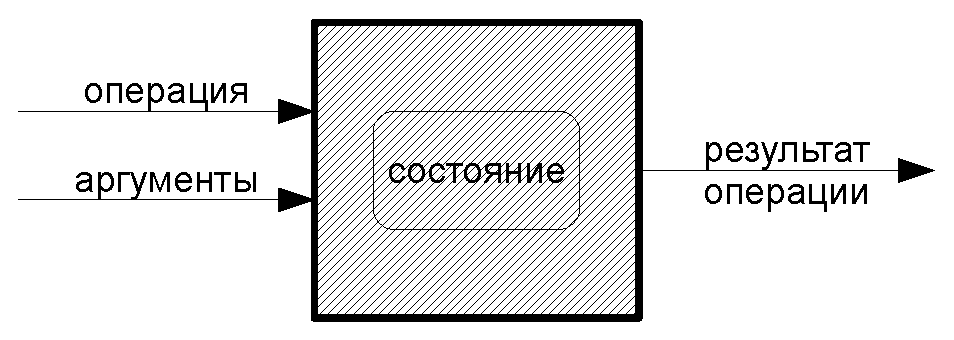
\includegraphics[width=0.7\textwidth]{rsl/machine}\\
  \caption{Конечноавтоматная модель программы}\label{fig:machine}
\end{figure}

По сравнению с реальной программной системой в такой модели нет таких понятий, как время выполнения операции и параллельное выполнение операций. Иными словами, <<операция>> аналогична функциям, в математическом смысле (функция --- как отображение входных данных к выходным, а не как подпрограмма). Но хотя нет понятия времени выполнения операции, есть понятие последовательности операций над системой.

Однако в этой модели выдача результата-значения  (как в примере с возведением в квадрат числа 2) не является обязательной и однозначной. А именно,
\begin{enumerate}
	\item на входное воздействие модель может ответить тем, что она перестает выдавать ответы вообще (<<зацикливается>>);
	\item на одни и те же входные воздействия модель может выдать различные ответы (модель недетерминирована);
	\item модель может ничего не ответить на входное воздействие в виде результата, но при этом может оказать \emph{побочный эффект}, и после этого продолжать выдавать ответы на следующие входные воздействия.
\end{enumerate}


\section*{Задачи}
	\zhead{Для следующих программ и программных систем привести несколько примеров конечноавтоматных моделей; какие возможны реализации этих систем, более мощные, чем конечные автоматы?}
		\z Стек.
		\z Почтовый клиент (например, Mozilla Thunderbird или веб-клиент Gmail).
		\z Электронный будильник.
		\z Компьютерная игра <<крестики-нолики>>.
		\z Подсистема работы с вкладками в веб-браузере.
		\z Веб-сайт микроблога (например, Twitter).
		\z Компиляторы gcc.
		\z Игровой веб-сервер для игры в покер. 

\section{Понятие корректности конечноавтоматных моделей программ}

просто "на словах" понятие корректности

зачем нужно формально записывать свойства корректности (чтобы автоматизировать проверку на однозначность, непротиворечивость, полноту? проверку соответствия разных моделей, проверку соответствия коду)

зачем нужен сам язык спецификации (зачем его надо изучать)

\section*{Задачи}
Сформулировать словесно, зачем нужно для пользователя, какие задачи решает """нечто""" (какой-нибудь компонент, алгоритм, ...) Т.е. это попытка посмотреть не с операционной, а декларативной точки зрения на программу

вычленить и сформулировать словами по-русски, например, для игры судоку в Ubuntu

пытаемся описать сложное решение и начинаем перечислять пути его получения (результат - то, что получено этим путем), потом еще путь, и еще и еще, в результате можем описать не то. Надо попытаться подумать "в общем случае".

\section{Сигнатура конечноавтоматной модели}

%сказать про то, как задавать "интерфейс" модели (как задавать список операций, как задавать состояние, про раздел value и раздел аксиом, в котором будут свойства). Целые числа, примеры моделей с целыми числами и примеры свойств в таких моделях.

Для фиксации рассматриваемых в курсе моделей программ будем пользоваться языком спецификации RSL (Rigorous Approach to Industrial Software Engineering Specification Language). Сейчас рассмотрим синтаксис описания моделей в этом языке. Это описание должно содержать как минимум список операций и список типов аргументов и типов результатов, для каждой операции должна быть указана сигнатура (имя операции, список типов аргументов, список типов результатов операции).

Описание модели без указания операций и типов:

\begin{lstlisting}
scheme MODEL_NAME = class

end
\end{lstlisting}

Описание операций и типов помещается между словами \textbf{class} и \textbf{end}. Описание типа очень простое:

\begin{lstlisting}
scheme STACK = class

type Stack
type Element

end
\end{lstlisting}

Можно объединить объявления типов Stack и Element так:

\begin{lstlisting}
scheme STACK = class

type Stack, Element

end
\end{lstlisting}

За каждым из таких типов закреплено некоторое множество значений и операторы сравнения на равенство/неравенство.

Операции описываются с указанием их имени, типов аргументов и типов результатов. Если типов несколько, они пишутся через символ $\times$. Порядок типов важен. Так описываются операции \emph{в аппликативном стиле}:

\begin{lstlisting}
scheme STACK = class
type Stack, Element

value push : Stack >< Element -~-> Stack

value pop : Stack -~-> Stack >< Element

end
\end{lstlisting}

Внимательный читатель спросит, зачем нужно 2 аргумента для того, чтобы поместить данные в стек? Или, если я ходу достать элемент с вершины стека, зачем я должен передавать еще какой-то аргумент? Дело как раз в аппликативном стиле. В нем мы обязаны передавать полностью всю информацию, которой будет пользоваться операция и какой информацией операция будет отвечать. Полностью --- значит, настоящие аргументы (например, те данные, которые надо положить в стек), состояние окружения модели (если это важно для ее функционирования) и внутреннее состояние модели! В данном случае окружение влияния не оказывает, а внутреннее состояние имеется и его мы указали в качестве дополнительных аргументов (Stack в аргументах и результатах операций).

Как отмечалось ранее, модель может <<зацикливаться>> ~\footnote{на деле модель не зацикливается, это слово выбрано для сокращения ситуации, когда модель перестает отвечать на входные воздействия}, может отвечать недетерминированно. Будем называть операцию модели  \emph{тотальной}, если по этой операции модель не <<зацикливается>> и ведет себя детерминированным образом. Для того, чтобы указать в модели, что некая операция является тотальной, нужно поставить в ее сигнатуре стрелку $\rightarrow$. В прошлом примере тотальной операцией должна быть операция push, а про операцию pop нельзя сказать, что она должна быть тотальной:
\begin{lstlisting}
scheme STACK = class
type Stack, Element

value
	push : Stack >< Element -> Stack,
	pop : Stack -~-> Stack >< Element
end
\end{lstlisting}

Заметим, что указать в операции, что она не должна быть тотальной, нельзя (операция либо только тотальная как push, либо всякая как pop). В последнем примере показано, как задать несколько операций в одной секции \textbf{value}.

Операции push и pop получают аргумент типа Element <<от пользователя>>, а аргумент типа Stack является одним из результатов других push и pop. Но рано или поздно должен найтись, грубо говоря, <<самое старое>>, <<первоначальное>>, значение в типе Stack для операций push или pop (это значение не представимо в виде результата push или pop, для его представления нужно иное средство). Для стека таким <<первоначальным>> значением является пустой стек. Добавим его в модель, такое значение является константой:

\begin{lstlisting}
scheme STACK = class
type Stack, Element

value
	empty : Stack,
	push : Stack >< Element -> Stack,
	pop : Stack -~-> Stack >< Element
end
\end{lstlisting}

\section*{Задачи}

описать сигнатуры операций над моделями, рассмотренными в предыдущих задачах. Указать требование тотальности операций, если операция должна быть тотальной.

\section{Предопределенные типы}

\textbf{Int}, \textbf{Nat}, \textbf{Real}, \textbf{Bool}, \textbf{Char}, \textbf{Text}, \textbf{Unit}.

Тип \textbf{Int} содержит в себе все возможные целые числа. Ограничений на их значения (типа MAXINT) нет.

Тип \textbf{Nat} содержит число 0 и все возможные положительные целые числа. Ограничений сверху на их значения нет. Тип поддерживает все операции, определенные для типа \textbf{Int}. Неограниченные целые числа необходимы для того, чтобы представлять такие заранее неограниченные величины как количества элементов, время (как количество единиц времени).

Тип \textbf{Real} содержит в себе все возможные вещественные числа. Важно понимать, что эти числа являются математической абстракцией тех вещественных чисел, которые представимы в архитектуре компьютера. Тип \textbf{Real} --- это те числа, с которыми работают математики. Следовательно, они включают и все вещественные числа, представимые в какой-угодно архитектуре компьютера. Например, в этом типе есть число <<квадратный корень из двух>>.

Тип \textbf{Bool} содержит булевские значения \textbf{true} и \textbf{false}.

Тип \textbf{Char} содержит все возможные отдельные символы. Этот тип не привязан ни к одной из кодировок (поскольку этот тип --- лишь математическая абстракция). Этот тип содержит все мыслимые символы. Поэтому не определена операция получения <<кода символа>>, привычная для многих языков программирования.

Тип \textbf{Text} является массивом символов (о массивах см.ниже).

Тип \textbf{Unit} является специальным и используется для ограниченного количества случаев (см.ниже). Основное применение --- то же, какое имеет ключевое слово \texttt{void} в сигнатурах функций языка Си.

\head{Операции над встроенными типами}
Арифметические:
\begin{lstlisting}
value
  +: Int >< Int -> Int,
  -: Int >< Int -> Int,
  *: Int >< Int -> Int,
  /: Int >< Int -~-> Int,
  \: Int >< Int -~-> Int,
  **: Int >< Int -~-> Int,
  abs: Int -> Nat,
  real: Int -> Real,

  +: Real >< Real -> Real,
  -: Real >< Real -> Real,
  *: Real >< Real -> Real,
  /: Real >< Real -~-> Real,
  **: Real >< Real -~-> Real,
  abs: Real -> Real,
  int: Real -> Int,

  <: Int >< Int -> Bool,
  <=: Int >< Int -> Bool,
  >: Int >< Int -> Bool,
  >=: Int >< Int -> Bool,

  <: Real >< Real -> Bool,
  <=: Real >< Real -> Bool,
  >: Real >< Real -> Bool,
  >=: Real >< Real -> Bool,

  ~: Bool       -> Bool,
  /\: Bool >< Bool -> Bool,
  \/: Bool >< Bool -> Bool,
  =>: Bool >< Bool -> Bool,
\end{lstlisting}

Для любого типа определены операции сравнения на равенство:
\begin{lstlisting}
type T
value
  = : T >< T -> Bool,
  ~= : T >< T -> Bool
\end{lstlisting}

Порядок вычисления операций строго определен: сначала первый аргумент, затем, если необходимо, второй и т.д.

Логика короткая. Это означает, например, что если первый аргумент конъюнкции равен \textbf{false}, то второй аргумент не вычисляется и вся конъюнкция принимает значение \textbf{false}.

\section*{Задачи}

%TODO
то, что было в задачнике Кузьменковой

\section{Императивное описание операций}

Теперь обратимся к тому, как описать \emph{псевдокод операций}. Для демонстрации сразу приведем пример записи псевдокода алгоритма Евклида:

\begin{lstlisting}
scheme GCD = class

variable a: Nat, b : Nat

value
  euclid: Unit -~-> write a, b Nat
  euclid() is
     while a > 0 /\ b > 0 do
        if a > b then a := a - b
        else b := b - a end
     end;
     if a = 0 then b else a end
end
\end{lstlisting}

Еще один, на этот раз рекурсивный, вариант псевдокода алгоритма Евклида:

\begin{lstlisting}
scheme GCD = class

value
  euclid: Nat >< Nat -~-> Nat
  euclid(a, b) is
		if a = 0 then b 
		elsif b = 0 then a
		elsif a > b then euclid(a - b, b)
		else	euclid(a, b-a)
		end
end
\end{lstlisting}

Как видно, язык RSL предлагает использовать такие известные понятия как глобальные переменные, присваивание, последовательности операторов, условный оператор \textbf{if-then-elsif-else-end}, операторы циклов (\textbf{while}), но это ещё не всё. Заметьте, если операции нужно получить доступ к переменной, то это надо указать в сигнатуре операции при помощи ключевого слова \textbf{write} (и \textbf{read}, см. ниже).

\head{Глобальные переменные}
Переменные, определенные вне функции, являются глобальными.
Каждая глобальная переменная должна быть определена в разделе \textbf{variable}, а в сигнатуре функции должен быть указан режим работы функции с переменной: <<только по чтению>> или <<по записи-чтению>>. Функции разрешено оперировать лишь с теми глобальными переменными, которые указаны в сигнатуре. Обращаться к глобальным переменным (даже просто по чтению), не упомянутым в сигнатуре, запрещается. Например,
\begin{lstlisting}
scheme S1 = class
variable status : Text
value
  init : Unit -~-> write status Unit
  init() is (status := "initialized")	
end
\end{lstlisting}

Функция \texttt{init} не имеет аргументов --- для указания этого факта перед стрелкой в сигнатуре функции указан тип \textbf{Unit}. Также у функции нет и результатов. Однако функции разрешено иметь побочный эффект в виде изменения значения глобальной переменной \texttt{status}.

Еще пример:
\begin{lstlisting}[escapechar={|}]
scheme S2 = class
variable status : Text
value
  |is\_initialized| : Unit -~-> read status Bool
  |is\_initialized|() is
	(status = "initialized")	
end
\end{lstlisting}

Здесь глобальная переменная лишь читается в функции, поэтому в сигнатуре переменная \texttt{status} указана с модификатором \textbf{read}.

Можно указать в сигнатуре, что функция может читать или изменять \textbf{любую} глобальную переменную. В этом случае надо после слов \textbf{write} или \textbf{read} вместо имени переменной написать ключевое слово \textbf{any}.

\head{Тело функции}
Язык RSL позволяет задавать выполнение функции в виде последовательности операторов, условного оператора и операторов цикла:
\begin{lstlisting}
scheme S3 = class
	variable a, b : Nat
	value
		swap : Unit -> write a, b Unit
		swap() is
		(
			a := a + b ;
			b := a - b ;
			a := a - b ;
		)
end
\end{lstlisting}

Если функции нужно вернуть некоторое значение, последовательность операторов должна завершаться выражением, чей результат будет результатом работы функции:
\begin{lstlisting}
scheme S4 = class
	variable a, b : Nat
	value
		swap : Unit -> write a, b Nat
		swap() is
		(
			a := a + b ;
			b := a - b ;
			a := a - b ;
			a + b
		)
end
\end{lstlisting}

Среди операторов, объединяемых в последовательность операторов, может быть присваивание, вызов функций, чей возвращаемый тип \textbf{Unit}, условный оператор, оператор цикла.

Условный оператор:
\begin{lstlisting}
scheme S4 = class
	variable a, b : Nat, s : Text
	value
		max : Unit -> read a, b, write s Nat
		max() is
		(
			if a > b then
				s := "first";
				a
			else
				s := "second";
				b
			end
		)
end
\end{lstlisting}

Условный оператор с веткой \emph{elsif}:
\begin{lstlisting}
scheme S4 = class
	variable x : Int, s : Text
	value
		Abs : Unit -> read x, write s Nat
		Abs() is
		(
			if x > 0 then
				s := "positive";
				x
			elsif x = 0 then
				s := "zero";
				0
			else
				s := "negative";
				-x
			end
		)
end
\end{lstlisting}


Операторы циклов (while, do-until и for):

\begin{lstlisting}
variable a: Nat, b : Nat
value
  euclid: Unit -~-> write a, b Nat
  euclid() is
     while a > 0 /\ b > 0 do
        if a > b then a := a - b
        else b := b - a end
     end;
     if a = 0 then b else a end
\end{lstlisting}

\begin{lstlisting}
variable n: Nat, x : Nat
value
  digits: Unit -~-> write n, x Nat
  digits() is
     n := 0;
     do n := n + 1; x := x / 10
     while x = 0;
     n
\end{lstlisting}

\begin{lstlisting}
variable sum : Nat
value
  sumN: Nat -~-> write sum Unit
  sumN(n) is
	sum := 0;
        for i in <.1 .. n.> do
	  sum := sum + i
	end;
\end{lstlisting}

\begin{lstlisting}
variable sum : Nat
value
  sumN: Nat -~-> write sum Unit
  sumN(n) is
	sum := 0; i := 0;
    do
      i := i + 1;
      sum := sum + i
    until i = n	end;
\end{lstlisting}

Способов прервать цикл типа break в RSL нет.

Локальные переменные:
\begin{lstlisting}
variable a: Nat, b : Nat
value
  euclid: Unit -~-> read a, b Nat
  euclid() is
   local variable a1: Nat := a,
                  b1: Nat := b in
     while a1 > 0 /\ b1 > 0 do
        if a1 > b1 then a1 := a1 - b1
        else b1 := b1 - a1 end
     end;
     if a1 = 0 then b1 else a1 end
   end
\end{lstlisting}

%%TODO есть ли неявный LET в императивном стиле ?

\head{Массивы}
Следующая функция использует массив целых чисел:
\begin{lstlisting}
value sort: Int-list -~-> Int-list
\end{lstlisting}

Обращение по индексу делается так: A(1). Нумерация индексов \textbf{с единицы}. Операция \textbf{len} возвращает текущую длину массива. Массивы в RSL могут изменять длину (путем операции конкатенации). Индекс не должен иметь большее значение, чем длина массива, и меньшее, чем 1. Синтаксис RSL запрещает изменять значения отдельных элементов массивов (например, так: <<A(i) := i>>), можно только строить новые массивы целиком (например, вместо <<A(i) := e>> можно писать <<A := $\langle$ if k=i then e else A(k) end | k in $\langle$1 .. \textbf{len} A$\rangle$ $\rangle$>>).

\begin{lstlisting}
value
  sum: Int-list -~-> Int
  sum(ls) is
    local variable s : Int := 0 in
       for i in <.1 .. len ls.> do
             s := s + ls(i)
       end;
       s
    end;
\end{lstlisting}


Эту же функцию, суммирующую элементы массива, можно записать и без использования индексов:
\begin{lstlisting}
value
  sum: Int-list -~-> Int
  sum(ls) is
    local variable s : Int := 0 in
       for l in ls do
             s := s + l
       end;
       s
    end;
\end{lstlisting}

Тип \textbf{Text} является массивом из \textbf{Char}.

Операция \textbf{tl} возвращает <<подмассив>> --- от второго элемента до последнего элемента исходного массива. Операция определена только для непустых массивов. Пустой список обозначается символом <..>. Тем самым функцию sum можно записать следующим образом с использованием рекурсии:
\begin{lstlisting}
value
  sum: Int-list -~-> Int
  sum(ls) is
    if ls = <..> then 0
    else ls(1) + sum(tl ls) end
\end{lstlisting}


\head{Структуры}
\begin{lstlisting}
type FIO ::
         name : Text
         surname : Text
value
   hello: FIO -~-> Text
   hello(fio) is
      "Hello, " ^ name(fio) ^
           "  " ^ surname(fio) ^ "!"
\end{lstlisting}

Обращение к полю делается в виде вызова функции с именем поля.

\begin{lstlisting}
type FIO ::
         name : Text
         surname : Text
value
   new_fio: Text >< Text -~-> FIO
   new_fio(n,sn) is mk_FIO(n,sn)
\end{lstlisting}

Создание структуры делается с помощью функции с предопределенным именем. Это имя начинается с <<mk\_>>, за которым идет имя типа структуры. В скобках подряд перечисляются выражения, дающие значения полям новой структуры.

\head{Перечисления (enumeration)}
\begin{lstlisting}
type Color = red | blue | white | green
value
  from_rus : Color -~-> Bool
  from_rus(c) is c = red \/ c = blue \/ c = white
\end{lstlisting}

\head{Указатели}
RSL не содержит встроенных механизмов для задания алгоритмов, работающих с указателями и работающих с динамической памятью.

    \section*{Задачи}

    % !Mode:: "TeX:UTF-8"
\zhead{<<Эффект>> операций}
%% приходится добавлять обсерверы, чтобы полностью описать эффект функции

\z В~\cite{tanenbaum_os} описаны операции с файлами, среди них описана операция Create следующим образом: <<\textsf{Create} (создание). Файл создается без данных. Этот системный вызов объявляет о появлении нового файла и позволяет установить некоторые его атрибуты.>> Напишите алгебраическую спецификацию файловой подсистемы с этой операцией. Естественно, вам понадобится сигнатура этой операции. Вот она:  \texttt{int creat(char *path, int mode)}, параметр \texttt{path} содержит полное или относительное имя файла, параметр \texttt{mode} устанавливает атрибуты прав доступа различных категорий пользователей к новому файлу при его создании (если файл уже существовал, то новый не создается), операция возвращает значение файлового дескриптора для открытого файла при нормальном завершении и значение -1 при возникновении ошибки.

Решение:
\begin{lstlisting}
scheme FS = class
  type Path, Mode, FID, FS
  value
        creat : FS >< Path >< Mode -~-> FS >< FID,
        size: FS >< FID -~-> Nat,
        known: FS >< Path -> Bool,
        access: FS >< FID -~-> Mode,
        first: FS >< FID -> FS  first(a,b) is a
  axiom forall path: Path, mode: Mode, fs: FS :-
        size(creat( path, mode, fs )) is 0,
        known(first(creat( path, mode, fs )), path),
        access(creat( path, mode, fs)) is mode
end
\end{lstlisting}
Обратите внимание, что
\begin{enumerate}
  \item для описания эффекта функции \texttt{creat} были введены дополнительные операции-обсерверы;
  \item аксиомы напрямую выражают текст, описывающий операцию \texttt{creat} --- аксиомы формализуют \emph{требования} на эту операцию.
\end{enumerate}
Ответьте на следующие вопросы:
\begin{enumerate}
  \item эта спецификация неполная, почему? является ли она противоречивой? как, добавив 1 аксиому, полностью описать операцию known?
  \item имеют ли смысл сами по себе введенные дополнительные операции или они выполняют лишь вспомогательную для описания \texttt{creat} функцию?
  \item допустим, мы догадываемся, что Path = \textbf{Text}, а Mode = \textbf{Nat}; дополненная этим знанием спецификация, останется ли алгебраической ? станет ли полной ? останется ли непротиворечивой ? будет ли она соответствовать исходной постановке задачи ? не станет ли она допускать того, что не должно бы по условию ?
\end{enumerate}

\z В~\cite{tanenbaum_os} описаны операции с файлами, среди них описана операция Delete следующим образом: <<\textsf{Delete} (удаление). Когда файл уже более не нужен, его удаляют, чтобы освободить пространство на диске. Этот системный вызов присутствует в каждой операционной системе.>> Напишите алгебраическую спецификацию файловой подсистемы с этой операцией. Естественно, вам понадобится сигнатура этой операции. Вот она:  \texttt{void delete(const char *path)}, параметр \texttt{path} содержит абсолютный или относительный путь к файлу.

\z В~\cite{tanenbaum_os} описаны операции с файлами, среди них описана операция Open следующим образом: <<\textsf{Open} (открытие). Прежде чем использовать файл, процесс должен его открыть. Системный вызов open позволяет системе прочитать в оперативную память атрибуты файла и список дисковых адресов для быстрого доступа к содержимому файла при последующих вызовах.>> Напишите алгебраическую спецификацию файловой подсистемы с этой операцией. Естественно, вам понадобится сигнатура этой операции. Вот она:  \texttt{fid open(const char *path)}, параметр \texttt{path} содержит абсолютный или относительный путь к файлу.

\z В~\cite{tanenbaum_os} упомянут системный вызов mmap: <<Системный вызов mmap принимает на входе два параметра: имя фала и виртуальный адрес памяти, по которому операционная система отображает указанный файл. Для реализации отображения файлов на память изменяются системные внутренние таблицы.При обращении к памяти по адресу от 512 до 576К происходит прерывание из-за отсутствия страницы, обработчик которого предоставляет считанную в память страницу 0 файла.Если потом эта страница удаляется из памяти алгоритмом замены страниц, она записывается в соответствующее место файла.>>

%% понять, как описывать недопустимое поведение

%\zhead{Спецификация отношений <<многие-ко-многим>>}
%
%Алгебраические спецификации позволяют описать многие компоненты, осуществляющие отношение <<многие-ко-многим>>, совершенно не задумываясь о том, каким образом это отношение выразить чем-нибудь более известным (например, вспомните, сколько есть различных способов представления этого отношения для реляционной модели данных!)
%
%\z Специфицируйте компонент, отвечающий за хранение и модификацию данных о студентах Университета и спецкурсах. А именно, есть студенты, они добавляются в базу внутри этого компонента. Есть спецкурсы, которые также добавляются. Как-то студенты записываются на спецкурсы. Компонент позволяет

\zhead{Термы, конфлюэнтность}

\z Приведите несколько различных примеров типов и функций, удовлетворяющих спецификации:
\begin{lstlisting}
type E, S
value empty: S,
      add: S >< E -> S
axiom all e: E :- empty ~= add(empty,e)
\end{lstlisting}

\z Приведите несколько различных примеров типов и функций, удовлетворяющих спецификации:
\begin{lstlisting}
type E, S
value empty: S,
      add: S >< E -> S
axiom all e: E :- empty = add(empty,e)
\end{lstlisting}

\z Приведите несколько различных примеров типов и функций, удовлетворяющих спецификации:
\begin{lstlisting}
type E, S
value empty: S,
      add: S >< E -> S
axiom all e: E :- empty ~= add(empty,e),
all e: E :- empty = add(add(empty,e),e),
\end{lstlisting}

\z Приведите несколько различных примеров типов и функций, удовлетворяющих спецификации:
\begin{lstlisting}
type E, S
value empty: S,
      add: S >< E -> S
axiom all e: E :- empty ~= add(empty,e),
all e1,e2: E :- empty = add(add(empty,e1),e2),
\end{lstlisting}

\z Приведите несколько различных примеров типов и функций, удовлетворяющих спецификации:
\begin{lstlisting}
type E, S
value empty: S,
      add: S >< E -> S
axiom all e: E :- empty ~= add(empty,e),
all e1,e2: E :- empty ~= add(add(empty,e1),e2),
\end{lstlisting}

\z Приведите несколько различных примеров типов и функций, удовлетворяющих спецификации:
\begin{lstlisting}
type E, S
value empty: S,
      add: S >< E -> S
axiom all e1,e2: E :- add(empty,e1) = add(empty,e2)
\end{lstlisting}

\z Приведите несколько различных примеров типов и функций, удовлетворяющих спецификации:
\begin{lstlisting}
type E, S
value empty: S,
      add: S >< E -> S
axiom all e1,e2: E :- add(empty,e1) ~= add(empty,e2) pre e1 ~= e2,
all e1,e2: E :- add(empty,e1) = add(add(empty,e2),e1)
\end{lstlisting}




\section{Множества, списки, отображения}

Более мощные алгоритмы требуют более сложных структур данных. RSL содержит (в дополнение к уже рассмотренным массивам, структурам и перечислениям) средства для работы с множествами, списками и отображениями. 

% !Mode:: "TeX:UTF-8"


\head{Множества}
Множество -- это контейнер элементов одного типа, который обладает свойствами уникальности и неупорядоченности его элементов. Множества бывают конечными и бесконечными.

Типовое выражение для конечного множества: $typeexpr\Set$. Типовое выражение для бесконечного множества: $typeexpr\Infset$. Конечное множество -- подтип бесконечного множества.

Операции над множествами:
\begin{list}{}{}
\item $= : T\Infset \DP T\Infset \Fn \Bool$ -- сравнение на равенство
\item $\neq : T\Infset \DP T\Infset \Fn \Bool$ -- сравнение на не равенство
\item $\Union: T\Infset \DP T\Infset \Fn T\Infset$ -- объединение пары множеств
\item $\Union: T\Infset\Infset \Fn T\Infset$ -- объединение множества множеств
\item $\Inter: T\Infset \DP T\Infset \Fn T\Infset$ -- пересечение пары множеств
\item $\Inter: T\Infset\Infset \Fn T\Infset$ -- пересечение множества множеств
\item $\Minus: T\Infset \DP T\Infset \Fn T\Infset$ -- вычитание множеств
\item $\Isin: T \DP T\Infset \Fn \Bool$ -- проверка на принадлежность
\item $\NotIsin: T \DP T\Infset \Fn \Bool$ -- проверка на непринадлежность
\item $\SetL: T\Infset \DP T\Infset \Fn \Bool$ -- проверка вложения
\item $\SetG: T\Infset \DP T\Infset \Fn \Bool$ -- проверка вложения
\item $\SetLE: T\Infset \DP T\Infset \Fn \Bool$ -- проверка вложения
\item $\SetGE: T\Infset \DP T\Infset \Fn \Bool$ -- проверка вложения
\item $\Card: T\Infset \NonDetermFn \Nat$ -- количество элементов
($\Chaos$ для бесконечных множеств)
\end{list}

Обратите внимание на отсутствие операции выбора произвольного элемента из множества!

Только операция \textbf{card} дает целое число от множеств, т.е. любое целочисленное выражение над множествами будет мощностью некоторого множества.

Конструкторы множеств:
\begin{list}{}{}
\item (\emph{пустое множество}) \{\}
\item (\emph{перечисление}) \{0, 1, 2\} - множество, состоящее из трех целых чисел (не
натуральных!) - нуля, единицы и двойки.
\item (\emph{диапазон}) \{0..2\} -  то же, что и \{0, 1, 2\};
\{0..0\} $\Iden$ \{0\}, \{1..0\} $\Iden$ \{\}
\item (\emph{<<сокращенная запись>>}) $\{ expr\_with\_var | var : typeexpr
\SuchAs boolexpr\}$ (например, $\{2 \star n | n : \Nat \SuchAs n < 3
\}$, что эквивалентно \{0, 2, 4\})
\end{list}

\head{Списки}
Список -- это контейнер элементов одного типа, который обладает свойствами упорядоченности элементов. Для задания списка надо указать не только сами элементы, но и их порядок. Списки бывают конечными и бесконечными.

Типовое выражение для конечного списка: $typeexpr\List$. Типовое выражение для бесконечного списка: $typeexpr\Inflist$. Конечный список -- подтип бесконечного списка.

Операции:
\begin{list}{}{}
\item $=: T\Inflist \DP T\Inflist \Fn \Bool$ -- проверка на равенство
\item $\neq: T\Inflist \DP T\Inflist \Fn \Bool$ -- проверка на не равенство
\item $(.) : T\Inflist \DP \Int \NonDetermFn T$ -- взятие элемента по
индексу ($\Chaos$ для индекса, отсутствующего в списке, индексы
нумеруются \textbf{с единицы})
\item $\Concat: T\List \DP T\Inflist \Fn T\Inflist$ -- конкатенация списков
\item $\Hd: T\Inflist \NonDetermFn T$ -- головной элемент списка ($\Chaos$ для пустого списка)
\item $\Tl: T\Inflist \NonDetermFn T\Inflist$ -- хвостовая часть списка ($\Chaos$ для пустого списка)
\item $\Len: T\Inflist \NonDetermFn \Nat$ -- количество элементов списка ($\Chaos$ для бесконечного списка)
\item $\Elems: T\Inflist \Fn T\Infset$ -- множество элементов списка (без повторений!)
\item $\Inds: T\Inflist \Fn \Nat\Infset$ -- множество индексов элементов списка
\end{list}

Конструкторы списков:
\begin{list}{}{}
\item (\emph{пустой список}) $\LL\LR$
\item (\emph{перечисление}) $\LL 0, 1, 2 \LR$ - список, состоящий из трех целых чисел (не натуральных!) - нуля, единицы и двойки - в порядке увеличения.
\item (\emph{диапазон}) $\LL 0..2 \LR$ -  то же, что и $\LL 0, 1, 2 \LR$; $\LL 0..0 \LR \Iden \LL 0 \LR$, $\LL 1..0 \LR \Iden \LL\LR$
\item (\emph{<<сокращенная запись>>}) $\LL expr\_with\_var | var \In listexpr \SuchAs boolexpr\LR$ (например, $\LL 2 \star n | n \In \LL 0..2 \LR \LR$, что эквивалентно $\LL 0, 2, 4 \LR$)
\end{list}


\head{Отображения}
Отображение -- это множество пар элементов, у которого первые компоненты не повторяются. Отображения бывают конечными и бесконечными, детерминированными и недетерминированными (это те, в которых первые компоненты всё же могут повторяться в разных парах).

Типовое выражение для детерминированного отображения: $$typeexpr_1 \Map typeexpr_2$$ Типовое выражение для недетерминированного отображения: $$typeexpr_1 \NonDeterMap typeexpr_2$$

Операции:
\begin{list}{}{}
\item $=: (T_1 \Map T_2) \DP (T_1 \Map T_2) \Fn \Bool$ -- сравнение отображений на равенство
\item $\neq: (T_1 \Map T_2) \DP (T_1 \Map T_2) \Fn \Bool$ -- сравнение отображений на не равенство
\item $(.): (T_1 \Map T_2) \DP T_1 \NonDetermFn T_2$ -- взятие значения по индексу ($\Chaos$, если значение по этому индексу не
определено)
\item $\Dom: (T_1 \Map T_2) \Fn T_1\Infset$ -- \emph{область определения} отображения
\item $\Rng: (T_1 \Map T_2) \Fn T_2\Infset$ -- \emph{область значения} отображения
\item $\Upd: (T_1 \Map T_2) \DP (T_1 \Map T_2) \Fn (T_1 \Map T_2)$ -- обновление отображения
\item $\Union: (T_1 \Map T_2) \DP (T_1 \Map T_2) \Fn (T_1 \NonDeterMap T_2)$ -- объединение отображений
\item $\Minus: (T_1 \Map T_2) \DP T_1\Infset \Fn (T_1 \Map T_2)$ -- уменьшение отображения
\item $/: (T_1 \Map T_2) \DP T_1\Infset \Fn (T_1 \Map T_2)$ -- проекция отображения
\item $\Superp: (T_2 \Map T_3) \DP (T_1 \Map T_2) \Fn (T_1 \Map T_2)$ -- композиция отображений
\end{list}

Конструкторы отображений:
\begin{list}{}{}
\item (\emph{пустое отображение}) []
\item (\emph{перечисление}) $[0 \mapsto 1, 1 \mapsto 2]$ -- отображение, состоящий из двух пар целых чисел (не натуральных!) - из 0 в 1 и из 1 в 2.
\item (\emph{<<сокращенная запись>>}) $[expr_1\_with\_var \mapsto expr_2\_with\_var | var : typeexpr \SuchAs boolexpr]$ (например, $[n \mapsto n+1 | n : \Nat \SuchAs n < 3]$, что эквивалентно $[0 \mapsto 1, 1 \mapsto 2, 2 \mapsto 3]$)
\end{list}


\subsection*{Задачи}

\zhead{Вычислить выражения с множествами}

\z $\{1, 2\} = \{3, 1\}$
\z $\{1, 2\} = \{2, 1\}$
\z $\{1, 2, 1\} = \{2, 2, 1\}$
\z $\{1, 2\}~\Union~\{3, 4\}$
\z $\{1, 2\}~\Union~\{2, 3\}$
\z $\{1, 2\}~\Inter~\{3, 4\}$
\z $\{1, 2\}~\Inter~\{2, 3\}$
\z $\{1..30\}~\Union~\{10..-10\}$
\z $\{1..30\}~\Inter~\{10..-10\}$
\z $\{1..30\}~\Union~\{x~|~ x: \Int~\SuchAs~\Abs x < 11 \}$
\z $\{1..30\}~\Inter~\{x~|~ x: \Int~\SuchAs~\Abs x < 11 \}$
\z $\{x+10 ~|~ x: \Int \} = \{x ~|~ x: \Int\}$
\z $\{5*k + 2 ~|~ k : \Int \}~\Inter~\{3*k - 1 ~|~ k : \Int\}$
\z $\{5*k + 2 ~|~ k : \Int \}~\Minus~\{3*k - 1 ~|~ k : \Int\}$
\z $\{5*k + 2 ~|~ k : \Int \} \SetL \{3*k - 1 ~|~ k : \Int\}$
\z $\{5*k + 2 ~|~ k : \Int \} \SetGE \{3*k - 1 ~|~ k : \Int\}$
\z $\Not (\{1, 2\} \SetLE \{2, 1, 1\})$
\z $\Card \{1..30\}$
\z $\Card \{5*k + 2 ~|~ k : \Int~\SuchAs~k * k \Isin \{-10..10\}\}$
\z $\Card \{5*k + 2 ~|~ k : \Int~\SuchAs~k * k \Isin \{10..-10\}\}$
\z $\Card \{k*k - 2 * k ~|~ k : \Int~\SuchAs~k * k \Isin \{-10..10\}\}$
\z $\All x: \Nat ~\SuchAs~ x \Isin \{x ~|~ x : \Int\}$
\z $\All x: \Int ~\SuchAs~ x \Isin \{x ~|~ x : \Nat\}$


\zhead{Решите уравнения}

\z $\{1\} \Union x = \{\}$
\z $\{1\} \Union x = \{1\}$
\z $\{1\} \Union x = \{1, 2\}$
\z $\{1\} \Inter x = \{\}$
\z $\{1\} \Inter x = \{1\}$
\z $\{1\} \Inter x = \{1, 2\}$
\z $\{2, 1\} \Minus x = \{1\}$
\z $\Card~x = 0$
\z $\Card~x = 1$


\zhead{Какие из следующих выражений истинные}
Считайте, что свободные переменные располагаются под квантором
всеобщности

\z $(A \cup B) \setminus C = (A \setminus C) \cup (B \setminus C)$
\z $(A \setminus B) \cap C = (A \cap C) \setminus B$
\z $(A \cup B) \setminus C \Iden (A \setminus C) \cup (B \setminus C)$
\z $A \cup \{\} = A$
\z $\{\} \cup A = A$
\z $(A \cup B) \cap C = (A \cap C) \cup (B \cap C)$
\z $\Card \Nat < \Card \Int$
\z $\Card \Nat = \Card \Int$
\z $\Card \Nat > \Card \Int$
\z $\Card \Nat \Iden \Card \Int$
\z $\Card \{n ~|~ n:\Nat\} \Iden \Card \{n ~|~ n:\Int\}$


\zhead{Записать на RSL следующие множества}

\z Пустое множество;
\z Множество чисел 1, 2, 3 (а также множество чисел от 1 до 3);
\z Множество всех чётных чисел;
\z Множество всех чётных чисел, не превышающих 10 (привести в виде перечисления и нескольких различных сокращённых формах);
\z Множество всех простых натуральных чисел;
\z Множество всех пар взаимнопростых натуральных чисел;
\z Множество всех троек, в каждой из которых есть одинаковые элементы;
\z Множество всех степеней двойки, не превышающих 100 (привести в виде перечисления и нескольких сокращённых формах);
\z Множество всех IP-адресов класса А (B, C, D, E);
\z Множество всех точек плоскости, образующих
    \begin{enumerate}
    \item Прямую -- биссектрису I и III квадрантов;
    \item Правую полуплоскость;
    \item Нижнюю полуплоскость;
    \item Единичную окружность;
    \item Единичный круг;
    \item Единичный квадрат со сторонами, параллельными осям
    координат.
    \end{enumerate}

%\zhead{Построить явную спецификацию на RSL для следующих задач}
%
%В этих задачах, если удаётся, следует привести два варианта решения: с использованием сокращённой записи множества
%и с помощью рекурсии.
%
%\z Дано множество чисел. Вернуть множество квадратов чисел данного множества.
%\z Дано множество чисел. Вернуть множество чисел, представимых суммами каких-либо двух элементов исходного множества.
%\z Дано множество точек, заданных координатами в плоской декартовой системе координат. Получить проекцию этого множества на ось \textsc{Ox}.
%\z Дано множество всех простых чисел. Для данного числа вернуть множество его простых делителей, используя множество всех простых чисел.
%\z Дано множество чисел. Дано число. Существует ли подмножество данного множества чисел, сумма элементов которого, равна данному числу.
%\z Дано множество множеств. Вернуть множество всех элементов внутренних множеств.
%\z \textit{(Задача о рюкзаке)} Дано множество предметов. Каждый предмет имеет массу (массы заданы множеством пар предмет >< масса). Есть $n$ рюкзаков. Каждый рюкзак имеет вместимость $K$ кг. Распределить все предметы по рюкзакам, не превышая вместимости каждого рюкзака.
%\z Рабочая группа компьютеров задаётся IP-адресом (4 целых числа, каждое от 0 до 255) и маской (целое число от 0 до 32). Программа по данному заданию строит множество всех возможных в ней IP-адресов.


\zhead{Вычислить выражения со списками}
\z $\LL 1 \LR = \LL 1, 1 \LR$
\z $\LL 1, 2 \LR = \LL 3, 1\LR$
\z $\LL 1, 2\LR = \LL 2, 1\LR$
\z $\LL 1, 2, 3 \LR (2)$
\z $\LL 1 \LR (0)$
\z $\LL 1 \LR (1)$
\z $\LL 1, 2\LR \Concat \LL 3, 4\LR$
\z $\LL 1, 2\LR \Concat \LL 2, 3\LR$
\z $\LL x+10~|~x~\In~\LL 1, 2 \LR \LR = \LL x~|~x~\In~\LL 1 \LR \LR$
\z $\Hd \LL 1, 2, 3 \LR$
\z $\Tl \LL 1, 2, 3 \LR$
\z $\Len \LL 1, 2, 3 \LR$
\z $\Elems \LL 1, 2, 3 \LR$
\z $\Inds \LL 1, 2, 3 \LR$
\z $\Len \LL 1..30\LR$
\z $\Let~x = \LL 1, 2, 3\LR~\In~\Elems~x~\Inter~\Inds~x~\rslEnd$
\z $\Let~x = \LL 0, 1, 2\LR~\In~\Elems~x~\Inter~\Inds~x~\rslEnd$
\z $\Let~x : \Int\Inflist~\SuchAs~(\All i_1, i_2: \Nat~\SuchAs~\Card \{i_1, i_2\} = \Card \{x(i_1), x(i_2)\})\\\In~x~\rslEnd$
\z $\Let~x : \Int\Inflist~\SuchAs~(\All i_1, i_2: \Nat~\SuchAs~\Card \{i_1, i_2\} = \Card \{x(i_1), x(i_2)\})\\\In~\Elems~x~\Inter~\Inds~x~\rslEnd$
\z $\All x : T\Inflist~\SuchAs~x(0) = \Hd x$
\z $\All x : T\Inflist~\SuchAs~x(0) ~\Iden~ \Hd x$

\zhead{Решите уравнения}
\z $\LL 1 \LR \Concat x  = \LL 1 \LR$
\z $\LL 1 \LR \Concat x  = \LL 1, 2, 3 \LR$
\z $\LL 1 \LR \Concat x  = \LL 3, 2, 1 \LR$
\z $\Tl x = \LL 1 \LR$
\z $\Hd x = 1$
\z $x \Concat \Tl x = x$
\z $\Tl x = \LL \Hd x \LR$
\z $\Elems x = \Inds x$
\z $\Elems~\Tl x = \Elems x$
\z $\Len x = \Card \Elems x$
\z $\Len x = \Card \Inds x$
\z $\Len x \Iden \Card \Inds x$


\zhead{Записать на RSL следующие выражения}

\z Пустой список;
\z Список из чисел 1, 2, 3 (попробуйте привести как можно больше различных решений);
\z Список всех простых натуральных чисел в порядке увеличения их значения;
\z Список всех пар взаимнопростых натуральных чисел в порядке увеличения их суммы;
\z Список номеров групп 5го курса факультета ВМиК МГУ в порядке увеличения номера группы;
\z Количество простых чисел от 1 до 10 (тремя различными способами).

%\zhead{Напишите явные спецификации следующих функций}
%
%\z Определить, является ли бесконечным данный список.
%\z Вычислить длину списка без использования функции $\Len$.
%\z Вычислить сумму элементов списка.
%\z Вычислить произведение элементов списка.
%\z Дан список. Построить список из элементов исходного списка, элементы которого идут в обратном порядке по отношению к исходному списку
%\z Дана строка и символ. Определить, встречается ли символ в данной строке (предложить два различных способа решения).
%\z Дана строка. Определить самый часто встречающийся в ней символ.
%\z Отсортировать данный список вещественных чисел в порядке возрастания.
%\z Построить список всех целых чисел в порядке неубывания модуля.
%\z Определить $\sup$ списка вещественных чисел (в случае конечного списка это будет и максимум).
%\z Выдать число, не встречающееся в данном списке.
%\z Дан список чисел. Построить по нему список квадратов, расположив элементы
%    \begin{enumerate}
%    \item с сохранением порядка исходного списка
%    \item в порядке убывания модуля
%    \item так, чтобы не было трёх подряд чисел, расположенных в  порядке возрастания или убывания.
%    \end{enumerate}
%\z Дано натуральное число. Построить список степеней его простых делителей, в котором на местоположение степени есть её основание (а значение, соответственно, показатель).
%\z Дан список показателей степеней (местоположение -- основание степени). Построить соответствующее натуральное число.
%\z Дан список натуральных чисел, отличных от нуля. Вернуть список, в котором на месте №$i$ находится количество раз, которое $i$ встречается в исходном списке.
%\z Дано множество чисел. Построить из него список, расположив элементы множества
%    \begin{enumerate}
%    \item в порядке убывания
%    \item в порядке убывания модуля
%    \end{enumerate}
%\z Дан список чисел. Построить из него новый список, расположив элементы исходного списка
%    \begin{enumerate}
%    \item в порядке убывания
%    \item в порядке убывания модуля
%    \end{enumerate}
%\z Дан список из чисел. Построить из него множество, использовав все элементы данного списка.
%\z Дан множество пар (ключ, объект) и список ключей. Построить соответствующий ему список объектов. Считайте, что во множество пар ключи не повторяются.
%\z Дан список чисел. Можно ли суммой некоторых его элементов получить
%    \begin{enumerate}
%    \item четное число (для списка из целых чисел)
%    \item простое число (для списка из целых чисел)
%    \item целое число (для списка из вещественных чисел)
%    \end{enumerate}


\zhead{Упростить выражения}
\z $\langle x ~|~ x~\In~\langle \Card \{a..b\} \rangle \rangle$
\z $\langle c ~|~ c~\In~\langle 'a',~'b' \rangle \rangle$
\z $\langle c ~|~ c~\In~\langle '$ " $~' \rangle \rangle$
\z $\langle c ~|~ c~\In~\langle \rangle \rangle$

\newcommand{\Masha}{\mbox{\textrm{<<Маша>>}}}
\newcommand{\Sveta}{\mbox{\textrm{<<Света>>}}}
\newcommand{\Misha}{\mbox{\textrm{<<Миша>>}}}
\newcommand{\Slava}{\mbox{\textrm{<<Слава>>}}}
\newcommand{\Anna}{\mbox{\textrm{<<Аня>>}}}
\newcommand{\Petr}{\mbox{\textrm{<<Петя>>}}}
\newcommand{\Lesha}{\mbox{\textrm{<<Леша>>}}}
\newcommand{\Victor}{\mbox{\textrm{<<Витя>>}}}

\zhead{Вычислить}

\z $\map{n \mapsto 1}{n : \Nat \SuchAs n \Isin \{1..3\} }$
\z $\map{n \mapsto n}{n : \Nat \SuchAs n \Isin \{5..5\} }$
\z $\map{n \mapsto n+1}{n : \Nat \SuchAs n \Isin \{100..90\} }$
\z $\map{n \mapsto m}{n, m : \Nat \SuchAs n \backslash m = 0 \And m > 2}$
\z $\map{n \mapsto m}{n, m : \Nat \SuchAs n \Isin \{1..3\} \And m \Isin \{1..n\}}$
\z $\map{n \mapsto (p, q)}{n, p, q : \Nat \SuchAs n \Isin \{1..100\} \And p + q = n \And p \backslash q = 0}$
\z $[1 \mapsto 2,~2 \mapsto 3,~ 3 \mapsto 1] (3)$
\z $[1 \mapsto 2,~2 \mapsto 3,~ 3 \mapsto 1] (4)$
\z $[ \Masha \mapsto 30, \Sveta \mapsto 15, \Masha \mapsto 30] (\Masha)$
\z $[ \Masha \mapsto 30,  \Sveta \mapsto 15, \Masha \mapsto 10 ] (\Masha)$
\z $[1 \mapsto [1 \mapsto 1,~ 2 \mapsto 2,~ 3 \mapsto 3], 2 \mapsto [1 \mapsto 4,~ 2 \mapsto 5,~ 3 \mapsto 6]~]~ (2)~(1)$
\z $\Dom [3 \mapsto 1, 5 \mapsto 0, 2 \mapsto 88]$
\z $\Rng [3 \mapsto 1, 5 \mapsto 0, 2 \mapsto 88]$
\z $\Dom \map{n \mapsto 2 * n}{n : \Nat}$
\z $\Rng \map{n \mapsto 2 * n}{n : \Nat}$
\z $[1 \mapsto 20, 2 \mapsto 30] \Union [1 \mapsto 30, 2 \mapsto 20]$
\z $[1 \mapsto 20, 2 \mapsto 30] \Upd [1 \mapsto 30, 2 \mapsto 20]$
\z $[ \Misha \mapsto 170, \Slava \mapsto 200, \Victor \mapsto 195 ] ~\backslash \\ \{\Misha, \Petr\}$
\z $[ \Misha \mapsto 170, \Slava \mapsto 200, \Victor \mapsto 195 ] ~/ \\\{\Misha, \Petr\}$
\z Пусть Friend = $[\Misha \mapsto \Anna, \Anna \mapsto \Lesha, \Lesha \mapsto \Misha]$. Найти Friend $\Superp$ Friend. Какой смысл этого значения ?
\z $\Card~\Dom~[1 \mapsto 2, 1 \mapsto 3, 2 \mapsto 3]$
\z $\Dom ([10 \mapsto 100, 20 \mapsto 50] \Upd [20 \mapsto 60, 30 \mapsto 90])$
\z $\Card~\Rng~( [1 \mapsto 2] \Superp [3 \mapsto 2, 4 \mapsto 1] \Superp [1 \mapsto 2, 3 \mapsto 4])$

\zhead{Какие из следующих выражений истинны}

Если выражение ложно, привести контрпример и дополнительные ограничения на входящие переменные, чтобы условие стало верным. Считать, что все переменные стоят под кванторами всеобщности.

\z $\Dom~ (X \Union Y) \Iden \Dom X ~\Union~ \Dom Y$
\z $\Rng~ (X \Union Y) \Iden \Rng X ~\Union~ \Rng Y$
\z $\Dom~ (X \Upd Y) \Iden \Dom X ~\Upd~ \Dom Y$
\z $\Rng~ (X \Upd Y) \Iden \Rng X ~\Upd~ \Rng Y$
\z $X = Y ~\Impl~ \Dom X = \Dom Y$
\z $X \NEq Y ~\Impl~ \Dom X ~\NEq~ \Dom Y$
\z $X \NEq Y ~\Impl~ \Rng X ~\NEq~ \Rng Y$
\z $\Dom (X \backslash Y) ~\Iden~ (\Dom X) \backslash Y$
\z $\Dom (X / Y) ~\Iden~ Y$
\z $\Dom (X \Upd Y) ~\Iden~ \Dom X \Union Y$
\z $(X \Union Y) \Union Z ~\Iden~ X \Union (Y \Union Z)$
\z $(X \Upd Y) \Upd Z ~\Iden~ X \Upd (Y \Upd Z)$
\z $(X \Superp Y) \Superp Z ~\Iden~ X \Superp (Y \Superp Z)$
\z $X \Union Y ~\Iden~ Y \Union X$

\zhead{Записать на RSL следующие константы и определения типов}
\z Записать отображение -- перестановку первых $N$ натуральных чисел. Считать $N$ константой с sort-определением.
\z Записать отображение-<<сдвиг>> : [1 $\mapsto$ 2, 2 $\mapsto$ 3, ..., $N \mapsto$ 1]. Считать $N$ константой с sort-определением.
\z Записать отображение всех полных квадратов в своё основание. [1 $\mapsto$ 1, 4 $\mapsto$ 2, 9 $\mapsto$ 3, ...]
\z Записать отображение из любого натурального числа в его простой делитель.
\z Записать отображение любого натурального числа в большее его простое натуральное число. [1 $\mapsto$ 5, 2 $\mapsto$ 7, 3 $\mapsto$ 5, ...]
\z Записать отображение <<бесконечная перестановка>>.
\z Записать отображение любого натурального числа в своё <<зеркало>> -- число из цифр исходного числа, записанных в обратном порядке. [1 $\mapsto$ 1, ..., 12 $\mapsto$ 21, ..., 832 $\mapsto$ 238, ...]
\z Записать отображение любого текста в его реверсию. $[..., \mbox{\textrm{"стол"}} \mapsto \mbox{\textrm{"лотс"}}, \mbox{\textrm{"книга"}} \mapsto \mbox{\textrm{"агинк"}}, ...]$
\z Не меняя описания предыдущей константы, описать новое отображение любого текста, начинающегося с 'a', в его реверсию.
\z Записать тип <<Англо-русский словарь>> так, как Вы его представляете. Учтите, что слово может иметь несколько переводов.

%\zhead{Запишите спецификацию функций в явном виде}
%\z Подсчитать количество элементов в данном отображении, если оно
%    \begin{enumerate}
%    \item детерминированное
%    \item ${^\star}$ недетерминированное
%    \end{enumerate}
%\z По отображению \{[$a \mapsto b$]\} построить отображение \{[$a^2 \mapsto b^2$]\}.
%\z Дано отображение \Nat $\Map$ \Nat. Вернуть количество элементов, отображающих в 0.
%\z По данному отображению \{[$a \mapsto b$]\} построить отображение \{[$b \mapsto x$]\}, где $b$ - правая часть некоторого элемента исходного отображения, а $x$ - количество раз, которое $b$ встретилось в исходном отображении.
%\z Дано отображение \Nat $\Map$ \Nat. Вернуть количество различных элементов, в которые осуществляется отображение.
%\z Дано отображение \Nat $\Map$ \Real, представляющее основание и показатель степени в разложении числа на простые множители. Вернуть число, которое представлено таким отображением.
%\z Дано натуральное число. Построить по нему отображение \Nat $\Map$ \Real, представляющее основание и показатель степени в разложении его на простые сомножители.
%\z Дано отображение строк \{[$s \mapsto t$]\}. Оставить в нём только те элементы, левая часть которого начинается с $s_0$.
%\z Проверить, является ли данное отображение детерминированным.
%\z Проверить, является ли данное отображение конечным.
%\z Проверить, является ли данное отображение взаимнооднозначным.
%\z Проверить, есть ли в данном отображении элемент $x \mapsto y$, где $x$ -- наибольший из всех левых частей, а $y$ -- наименьший среди всех правых частей.
%\z Проверить, является ли данное отображение перестановкой.
%\z Проверить, является ли данное отображение перестановкой первых $N$ натуральных чисел.
%\z Дано отображение \{[$(x, y) \mapsto L$]\} ($L$ -- множество). Проверить, верно ли, что все элементы в $L$ не больше $y$ и не меньше $x$.
%\z Дано отображение. Построить его максимальное детерминированное подотображение.
%\z Реляционное отношение задано отображением $T \Map A \DP B \DP C$. Проверить, есть ли среди атрибутов $A$, $B$, $C$ возможные ключи. Домены атрибутов считать sort-определенными.
%\z Реализуйте функцию $lower$, переводящую символы в нижний регистр. Какова, по Вашему, будет сигнатура этой функции?


\subsection*{Схемы сокращения записи}

Язык RSL обладает достаточно богатыми возможностями для записи выражений. В данном параграфе предлагается освоить ряд приемов по получению более краткой записи выражений за счёт использования различных предопределенных операций над множествами, списками и отображениями.

\paragraph{схема пересечения}

$$x~\Inter~ \{f(t) ~|~ t:T\}$$ вместо $$\{a ~|~ a: X ~\SuchAs~ a \Isin x ~\And~ ( \Exists t: T  ~\SuchAs~ x = f(t) ) \}$$

\paragraph{схема вычитания-1}

$$x ~\Minus~ \{f(t) ~|~ t:T\}$$ вместо $$\{a ~|~ a: X ~\SuchAs~ a \Isin x ~\And~  \Not( \Exists t: T  ~\SuchAs~ x = f(t) ) \}$$

\paragraph{схема вычитания-2}

$$\{f(t) ~|~ t:T\} ~\Minus~ x$$ вместо $$\{a ~|~ a: X ~\SuchAs~ a \NotIsin x ~\And~ ( \Exists t: T  ~\SuchAs~ x = f(t) ) \}$$

\paragraph{схема выборки по ключам (на примере)}
Из исходного отображения выделить подотображение с определенными ключами:
$$t / \{1, 2\}$$ вместо $$[a \mapsto t(a) ~|~ a:X ~\SuchAs~ a \Isin \Dom x ~\And~ a \Isin \{1, 2\} ]$$

\paragraph{схема выборки по значению}
Из исходного отображения выделить подотображение с определенными значениями:
$$[1 \mapsto 1,~ 2 \mapsto 2] \Superp t$$ вместо $$[a \mapsto t(a) ~|~ a:X ~\SuchAs~ a \Isin \Dom x ~\And~ t(a) \Isin \{1,2\} ]$$

%(( all x:X :- ~exists y1, y2: X-set :- y1 ~= y2 /\ x isin y1 inter y2 )) можно записать короче:
%(( ~exists y1, y2: X-set :- y1 ~= y2 /\ y1 inter y2 ~= {} ))
%
%all x:X :- ~exists y:X-set :- x isin y ::::::: ~exists y:X-set :- y ~={} ::::::: all y:X-set :- y = {}

\paragraph{схема соединения (join)}
Для компактной записи выражений, где нужно <<соединение>> двух отображений (join), следует использовать композицию отображений (это ее основное практическое применение).



\subsection*{Задачи}

\zhead{Записать следующие выражения}

При записи решений стараться выбирать наиболее короткую запись.

\z Дано непустое множество натуральных чисел m и натуральное число x. Записать логическое выражение, истинное тогда и только тогда, когда x равен максимальному числу во множестве m.

\textbf{Решение:}

%\begin{lstlisting}
%x isin m /\ (all y: Nat :- y isin m => y <= x)
%\end{lstlisting}
%
%а теперь более короткое решение:

\begin{lstlisting}
x isin m /\ {0..x} >>= m
\end{lstlisting}

\z Дано непустое множество целых чисел m и целое число x. Записать логическое выражение, истинное тогда и только тогда, когда x равен максимальному числу во множестве m.

\z Дано непустое множество натуральных чисел m и натуральное число x. Записать логическое выражение, истинное тогда и только тогда, когда x равен минимальному числу во множестве m.

\z Дано непустое множество натуральных чисел m. Записать сумму элементов этого множества.

\textbf{Решение:}
\begin{lstlisting}
card {(x,y)| x, y : Nat :- x isin m /\ y < x}
\end{lstlisting}

\z Дано непустое множество целых чисел m. Записать сумму элементов этого множества.

\z Дано непустое множество натуральных чисел m. Записать произведение элементов этого множества.

\z Дан непустой список t, натуральное число x и значение y того же типа, каков тип элементов в t. Записать логическое выражение, истинное тогда и только тогда, когда x является индексом первого вхождения y в t.

\z Дан непустой список t, натуральное число x и значение y того же типа, каков тип элементов в t. Записать логическое выражение, истинное тогда и только тогда, когда x является индексом последнего вхождения y в t.

\z Дан непустой список t, натуральные числа x1 и x2 (x2 > x1) и значение y того же типа, каков тип элементов в t. Записать логическое выражение, истинное тогда и только тогда, когда x1 и x2 являются индексами двух подряд вхождений y в t.

\z <<особые фамилии>>. Дано множество <<фамилий>> t. Записать множество фамилий из t, оканчивающихся на <<ов>>.

\textbf{Решение:}
\begin{lstlisting}[escapechar={@}]
t inter {z ^ @"ов"@ | z: Text}
\end{lstlisting}

\z Даны две строки t1 и t2. Записать логическое выражение, истинное тогда и только тогда, когда t2 является подстрокой строки t1.

\z Дана строка t. Записать выражение, равное реверсу строки t.

\z Дано отображение m некоторого типа в тот же тип. Записать логическое выражение, истинное тогда и только тогда, когда это отображение является перестановкой.

\z Дано отображение db строк в целые числа, причем все целые числа разные (например, эти числа - это какие-нибудь хэш-значения строк). В db добавляется строка t и получается db2 (всё остальное соответствие строк и целых чисел из db сохраняется, добавляется новое без нарушения свойства различия целых чисел). Записать логическое выражение, определяющее db2.

\textbf{Решение:}
\begin{lstlisting}[escapechar={@}]
db2 \ {t} = db /\ t isin dom db2 /\ db2(t) ~isin rng db
\end{lstlisting}

Обратите внимание, что сразу два требования (что сохраняются все строки и сохраняется соответствие строк и целых чисел) записано в первом конъюнкте. Обратите также внимание, что хоть и неизвестно целое число, поставленное в соответствие строке t в db2, возможно записать ряд важных свойств отображения db2.

\z Игровое поле игры <<крестики-нолики>> задано следующим способом:
\begin{lstlisting}
type Cell == empty | cross | toe
type Nat3 = {| n: Nat :- n isin {1..3} |}
type Field = (Nat3 >< Nat3) -m-> Cell
\end{lstlisting}
Дано f --- значение в типе Field. Записать
\begin{enumerate}
  \item логическое выражение, истинное тогда и только тогда, когда в отображении f есть информация обо всех клетках поля;
  \item выражение, равное числу пустых клеток.
\end{enumerate}

\z\label{z:correct_graph} Граф задан отображением вершин во множество инцидентных им вершин:
\begin{lstlisting}
type V, G = V -m-> V-set
\end{lstlisting}
Такое представление будет считаться <<корректным>>, если каждая вершина встречается среди первых компонент отображения (при отсутствии инцидентных вершин значение в отображении для такой вершины будет пустым множеством). Записать логическое выражение, истинное тогда и только тогда, когда данная переменная g типа G является <<корректным>> представлением графа.

\z Дано <<корректное>> представление g графа (см. задачу~\ref{z:correct_graph}) и список вершин p. Записать логическое выражение, истинное тогда и только тогда, когда p является путём в графе g.

\z Дано <<корректное>> представление g графа (см. задачу~\ref{z:correct_graph}) и его вершина v. Записать выражение, равное множеству вершин, достижимых из v через не более одну промежуточную вершину.

\textbf{Решение:}

\begin{lstlisting}
g(v) union (g#g)(v)
\end{lstlisting}

чуть более длинный вариант:
\begin{lstlisting}
g(v) union union rng (g/g(v))
\end{lstlisting}

\z Дано <<корректное>> представление g графа (см. задачу~\ref{z:correct_graph}) и его вершина v. Записать выражение, равное множеству вершин, которым инцидентна v.


\z В таксопарке есть следующая база:
\begin{lstlisting}[escapechar={@}]
type @Водитель@, @Машина@, @Водители@ = @Водитель@ -m-> @Машина@
\end{lstlisting}
Дана b --- база водителей с машинами.
\begin{enumerate}
  \item Дана машина c. Найти всех водителей машины c.
  \item Найти множество всех различных машин.
  \item У таксопарка есть доступ к базе машин:
\begin{lstlisting}[escapechar={@}]
type @Машина@, @Цвет@, @Машины@ = @Машина@ -m-> @Цвет@
\end{lstlisting}
Дана m --- база машин с их цветами. Найти водителей, которые ездят на 'красных' машинах.
\end{enumerate}


\zhead{Спецификация алгоритмов со структурами данных\footnote{Алгоритмы взяты из книги~\cite{structures_algorithms}}}

В этих задачах требуется переписать приведенные классические алгоритмы работы со структурами данных на RSL. Следите за тем, чтобы спецификация оставалась <<читабельной>>. Вам пригодится конструкция <<неявный let>>.

\z <<Алгоритм Дейкстры>>. Алгоритм предназначен для решения задачи нахождения кратчайших путей в ориентированном графе с неотрицательными пометками вершин. Длина пути --- это сумма пометок входящих в него дуг. В приведенном псевдокоде ищутся пути от вершины 1, остальные вершины графа пронумерованы числами от 2 до n, V --- это множество чисел от 1 до n. C[i,j] дает пометку дуги из i в j, или $\infty$, если такой дуги нет. Результат помещается в переменную S.

\begin{verbatim}
S := {1};
for i := 2 to n do
  D[i] := C[1,i];
for i := 1 to n-1 do
begin
  выбор из множества V\S такой вершины w,
     что значение D[w] минимально;
  добавить w к S;
  for каждая вершина v из множества V\S do
    D[v] := min(D[v], D[w]+C[w,v])
end
\end{verbatim}

% алгоритм Флойда

\z <<Алгоритм Прима>>. Алгоритм предназначен для решения задачи нахождения остовного дерева минимальной стоимости. Остовное дерево содержит все вершины исходного графа, но возможно не все его дуги. В алгоритме V --- это множество вершин (множество чисел от 1 до n). Результат формируется в дереве T.

\begin{verbatim}
T := пустое дерево;
U := {1};
while U не равно V do
begin
  (u,v) --- ребро наименьшей стоимости такое, что
    u принадлежит U и v принадлежит V\U;
  добавить в T (u,v);
  добавить в U v;
end
\end{verbatim}

% алгоритм Крускала

% алгоритм Прима

% разные остОвные подграфы

% поиск подслов

  % with problems


\section{Эксплицитное и имплицитное описание функций}

Рассмотренный ранее способ описания операций (в виде псевдокода) был \emph{эксплицитным} (explicit, явным) способом описания, поскольку в нем было указано явно <<алгоритм>> вычисления функции. Однако, это не единственный способ описания функций в языке RSL.

\emph{Эксплицитным} назовем следующий способ описания функций:
\begin{lstlisting}
value
	funcname : T1 >< ... >< T2 -~-> T3 >< ... >< T4
	funcname(t1, ..., t2) is
		... 
\end{lstlisting}

Т.е. в эксплицитном способе после сигнатуры идет имя функции с формальными аргументами, далее символ $\Is$ и затем псевдокод функции. Стрелка в сигнатуре функции может быть любой.

\emph{Имплицитным} назовем следующий способ описания функции:
\begin{lstlisting}
value
	funcname : T1 >< ... >< T2 -~-> T3 >< ... >< T4
	funcname(t1, ..., t2) as (t3, ..., t4)
	post
		... 
\end{lstlisting}

В имплицитном способе после сигнатуры идет имя функции с формальными аргументами, далее слово \textbf{as}, далее формальные имена результатов, далее слово \textbf{post}, после которого идет логическое выражение над именами t1, ..., t2, t3, ..., t4 (стрелка в сигнатуре может быть любой). Т.е. в имплицитном способе описания задается предикат, который истинен на тех и только на тех значениях имен t1, ..., t2, t3, ..., t4, что t3, ..., t4 является правильным результатом функции funcname на аргументах t1, ..., t2. Например:
\begin{lstlisting}
value
	max : Nat >< Nat -> Nat
	max(a, b) as m
	post
		m = a /\ a > b
		\/ m = b /\ a <= b
\end{lstlisting}

Выражение после слова \textbf{post} будем называть \emph{поствыражением}. Функцию из последнего примера можно задать и другим поствыражением:
\begin{lstlisting}
value
	max : Nat >< Nat -> Nat
	max(a, b) as m
	post
		if a > b then m = a 
				else m = b
		end
\end{lstlisting}

Сравните эту запись с эксплицитной записью той же функции:
\begin{lstlisting}
value
	max : Nat >< Nat -> Nat
	max(a, b) is
		if a > b then a 
				else b
		end
\end{lstlisting}

Несмотря на то, что логика короткая, следующее определение задает другую функцию, нежели функцию из последнего примера (ответьте, почему):
\begin{lstlisting}
value
	max : Nat >< Nat -> Nat
	max(a, b) as m
	post
		m = a /\ a > b
		\/ m = b
\end{lstlisting}

В поствыражении могут встречаться <<вызовы>> других функций:
\begin{lstlisting}
value
	sum: Nat-list -> Nat
	sum(x) as s
	post
		if x = <..> then s = 0
		else s = sum(tl x) + hd x end
\end{lstlisting}

Вы уже заметили, насколько похожи эксплицитная и имплицитная запись функций. На самом деле если функция не использует глобальных переменных по чтению-записи, то эксплицитная запись может быть переписана в имплицитном виде очень просто: вместо возвращаемых значений запись равенство, как это было сделано в последних примерах.

Однако если функция использует глобальные переменные по чтению-записи, то поствыражение должно содержать описание побочного эффекта. Дело в том, что поствыражение нужно для описания результата функции, поэтому:
\begin{enumerate}
\item поствыражение не должно иметь побочного эффекта;
\item поствыражение пишется только для функций, которые завершаются и завершаются детерминированным образом.
\end{enumerate}
Итак, если исходная функция имеет побочный эффект, например
\begin{lstlisting}
variable
	a, b : Int
value
	swap : Unit -> write a, b  Unit
	swap() is
		local variable temp : Int := a in
			a := b;
			b := temp
		end
\end{lstlisting} 
то эквивалентное определение функции в имплицитном виде полностью сохраняет сигнатуру, а в поствыражение должно входить соотношение значений переменных до вызова функции и значений после вызова функции:
\begin{lstlisting}
variable
	a, b : Int
value
	swap : Unit -> write a, b  Unit
	swap()
	post
		a = b' /\ b = a'
\end{lstlisting}

Штрихованные переменные --- это значения переменных \textbf{до} вызова функции.

\section{Контрольная работа №1}

примеры задач


%старое \section{Функции в языках спецификации}
%старое  % !Mode:: "TeX:UTF-8"

\emph{Функция} в данном курсе будет пониматься точно так же, как она понимается в математике, а именно, как отображение одного множества на другое. Для простоты можно понимать функцию как совокупность пар (x, y). Функции могут быть однозначные и многозначные (или, на более привычном для программистов языке, детерминированными и недетерминированными), т.е. либо для каждого х есть не более одной пары (x, y), либо таких пар может быть несколько. Каждая функция обладает \emph{областью определения}, т.е. множеством всех x из пар (x, y).

В математике нет понятия <<вызвать функцию>>, есть понятие <<применить функцию>>. Скажем, пусть f --- функция, x' принадлежит области определения f. Тогда применение функции f к x' (обозначать это будем стандартным образом: <<f(x')>>) есть недетерминированный выбор всех таких y', что в f, как совокупности пар, есть пара (x', y').

Эти определения формализуют знакомое всем определение функций, в котором подчеркивается, что функция --- это лишь математический объект, это не процесс, функция (в данном курсе) не исполняется во времени (если так проще понимать, можно считать, что функции <<работают мгновенно>>) и у функций (в отличие, например, от функций в языке Си) есть область определения (функцию в языке программирования можно вызывать с любыми аргументами, которые допустимы согласно статической типизации).

Однако функциям можно сопоставить ряд понятий, знакомых любому программисту. Например, если абстрагироваться от вычислительных и временных свойств, то каждой функции на языке программирования соответствует осуществляемое ею \emph{отображение}, что и есть функция, как она определена в данном разделе. Другой пример: операции пользователя с системой также можно промоделировать при помощи таких функций (хотя напрямую в коде реализации системы таких функций может и не быть, отдельные части таких функций могут быть распределены по различным функциям в коде реализации).

С точки зрения формальных спецификаций нас в этом курсе будут интересовать свойства функций, способы задания свойств функций и способы получения (вывода) новых свойств из имеющихся. Важно понимать, что функция сама по себе есть некий объект с операцией применения, а спецификация функции --- это набор свойств функции (но не сама функция). Одному и тому же набору свойств может соответствовать несколько функций. И, наоборот, для одной функции можно сформулировать массу различных свойств.

Свойства функций поделим на 2 класса --- синтаксические и семантические свойства. Синтаксические свойства функции --- это, проще говоря, сигнатура функции (имя функции, количество и типы её параметров). Важно понимать, что именно при помощи сигнатуры функции задается область определения функции. А именно, все значения параметров, удовлетворяющие своим типам, образуют область определения функции.

Семантические свойства функции --- это свойства отображения входных данных на выходные, которое осуществляет функция. Семантические свойства задаются при помощи предикатов над значениями аргументов функции и значения функции при этих аргументах. Примеры семантических свойств функции для функции $f$ с одним аргументом типа $\Int$ (любое целое число) и результатом тоже типа $\Int$:

\begin{itemize}
  \item $f(0) = 0$ (утверждается значение функции при заданном значении её аргументов);
  \item $\All x: \Int ~\SuchAs~ f(x) = -f(-x)$ (нечетность функции);
  \item $\Exists x: \Int ~\SuchAs~ f(x) \equiv \Chaos$ (функция на каком-то значении аргумента зацикливается);
  \item $f(x) = x + 1$, если $x = 0, 1, 2, .., 10$ (частичное задание функции);
  \item $f(x) = x + 1$, если $x = 0, 1, 2, ..., 10$, $f(x) = 0$, иначе (полное задание функции);
  \item у функции $f$ 1 аргумент (синтаксическое свойство функции);
  \item $f(0)$ может равняться 0 или 1 (это свойство можно трактовать двояко - либо функция $f(x)$ ведет себя \emph{недетерминированно} при $x = 0$ и может вернуть число 0 или число 1 (т.е. при работе программы с такой функцией могут возникнуть оба значения), либо функция $f(x)$ ведет себя детерминированно при $x = 0$ и $f(0)$ равняется одному из чисел 0 или 1 (при работе программы с такой функцией может возникнуть только одно из чисел)).
\end{itemize}

Запись синтаксических свойств функции на языке RSL описана в предыдущем разделе. Для записи семантических свойств функций язык RSL предлагает пользоваться \emph{аксиомами}. Например, свойство $f(0) = 0$ будет записано следующим образом:

\begin{lstlisting}
value f: Int -~-> Int
axiom f(0) is 0
\end{lstlisting}

Свойство нечетности функции:
\begin{lstlisting}
value f: Int -~-> Int
axiom all x: Int :- f(x) is -f(-x)
\end{lstlisting}

Частичное определение функции можно дать следующим образом:
\begin{lstlisting}
value f: Int -~-> Int
axiom all x: Int :- x >= 0 /\ x <= 10 => f(x) is x+1
\end{lstlisting}

Но нагляднее будет воспользоваться \emph{\textbf{pre}-выражением}, ограничивающим область значений подкванторных переменных:
\begin{lstlisting}
value f: Int -~-> Int
axiom all x: Int :-
        f(x) is x + 1 pre x >= 0 /\ x <= 10
\end{lstlisting}

Полное определение можно дать с использованием одной аксиомы:
\begin{lstlisting}
value f: Int -~-> Int
axiom all x: Int :-
    f(x) is (if x >= 0 /\ x <= 10 then x+1 else 0 end)
\end{lstlisting}

или так:

\begin{lstlisting}
value f: Int -~-> Int
axiom all x: Int :-
    (x >= 0 /\ x <= 10 => f(x) is x + 1) /\
    ((x < 0 \/ x > 10) => f(x) is 0)
\end{lstlisting}

или с использованием двух аксиом:
\begin{lstlisting}
value f: Int -~-> Int
axiom
all x: Int :- f(x) is x + 1  pre x >= 0 /\ x <= 10,
all x: Int :- f(x) is 0  pre x < 0 \/ x > 10
\end{lstlisting}

можно воспользоваться конструкцией forall для сокращения количества кванторов всеобщности:
\begin{lstlisting}
value f: Int -~-> Int
axiom forall x: Int :-
    f(x) is x + 1  pre x >= 0 /\ x <= 10,
    f(x) is 0  pre x < 0 \/ x > 10
\end{lstlisting}

\head{Спецификация тотальных функций}

Если рассматривать однопроцессные однопотоковые невзаимодействующие с окружением программы, которые должны результативно завершаться (и только тогда такие программы имеют смысл), то про функции в программах можно говорить следующее:
\begin{itemize}
  \item на некоторых данных функция завершается;
  \item на некоторых данных функция завершается и ее результат детерминирован (т.е. будет точно таким же, если вызвать функцию с теми же аргументами и значениями глобальных переменных);
  \item на некоторых данных функция завершается и ее результат недетерминирован;
  \item на некоторых данных функция зацикливается (программа <<повисла>>);
  \item во время работы функция пытается выполнить недопустимую операцию (программа <<упала>>).
\end{itemize}

Для работы программы важно, чтобы ее функции не зацикливались и не <<падали>> как минимум на некотором <<нужном>> множестве входных данных (в противном случае этой функцией нельзя будет пользоваться). Аналогом таких функций в программах (которые не должны зацикливаться и <<падать>>) являются тотальные функции.

Будем называть функцию \emph{тотальной}, если в этой функции каждому значению из области определения соответствует единственное значение. На RSL это определение может быть записано так\footnote{Такое часто встречающееся определение тотальной функции не является верным: $\All x:X ~\SuchAs~ \ExistsOne y:Y ~\SuchAs~ f(x) ~\Is~ y$, поскольку выражение $f(x)$ потенциально может содержать побочный эффект, а выражение $y$ не содержит побочного эффекта, поэтому эти выражения не могут быть эквивалентными}:
$$\All x:X ~\SuchAs~ \ExistsOne y:Y ~\SuchAs~ \AllStates~ (f(x) = y)$$


Переводя это на язык функций в языках программирования, можно сказать, что таким функциям в спецификации следует писать тотальную функцию, если для исходной функции на всех значениях входных параметров, соответствующих их типам, выполнены оба следующих свойства:
\begin{enumerate}
  \item она результативно завершима (т.е. не зацикливается и не падает ни при каком значении аргументов и глобальных переменных);
  \item её результат детерминирован (если функция вызывается в разное время с теми же аргументами и в том же состоянии глобальных переменных, то она возвращает одинаковые значения и одинаковым образом изменяет глобальные переменные).

%  \item она всюду определена (функция возвращает какое-либо значение на каждом значении аргументов и глобальных переменных, согласно их типам);
\end{enumerate}

Тотальность функции является синтаксическим свойством и входит в сигнатуру функции. А именно, в функции, которая должна быть тотальной, вместо стрелки $\NonDetermFn$ ставится стрелка $\Fn$. Однако спецификация может не содержать требования функции быть тотальной, но в коде реализации эта функция в действительности будет тотальной. Иначе говоря, \textit{стрелка $\NonDetermFn$ в сигнатуре не означает, что функция не является тотальной}. Стрелка $\NonDetermFn$ означает, что функция может быть какой угодно, как тотальной, так и нетотальной.

\head{Полное определение функции. Случай недоспецификации}

Набор синтаксических и семантических свойств будем называть \emph{определением} функции, если семантические свойства дают возможность однозначно судить о значениях функции при всех входных данных, допустимых сигнатурой функции (грубо говоря, спецификация функции является определением, если этой спецификации соответствует единственная функция, и поэтому можно даже вычислить значение функции при любом заданном значении входных параметров; единственная функция не означает единственного значения при каком-либо аргументе функции, т.е. существуют спецификации, дающие определение недетерминированных функций).

Спецификацию функции будем называть \emph{полной}, если она позволяет сделать вывод о значении функции при \textbf{каждом} значении ее аргументов и глобальных переменных (т.е. если эта спецификация дает определение функции). Остальные спецификации будем называть \emph{неполными}, или \emph{частичными}. При частичном задании удобно использовать \textbf{pre}-выражения (примеры были даны выше).

Пример полной спецификации:
\begin{lstlisting}
value f: Int >< Int -> Int
axiom forall x, y: Int :-
    f(x, y) is x + y pre x > y,
    f(x, y) is x - y pre x <= y
\end{lstlisting}
При каждом значении пары (x, y) в этой спецификации задано значение функции f. Тем самым эта спецификация функции f является полной.

Пример неполной спецификации:
\begin{lstlisting}
value f: Int >< Int -> Int
axiom forall x, y: Int :-
    f(x, y) is x + y pre x > y
\end{lstlisting}
Из этой спецификации можно сделать вывод о значении функции f на тех парах (x, y), где x > y, но нельзя сделать вывод  о значениях функции f на остальных парах. Тем самым, эта спецификация функции f является неполной. Эту спецификацию можно \emph{доопределить} до полной спецификации бесконечным числом способов (не нарушая требования тотальности функции f). Спецификацию, в которой есть неполная спецификаций какой-либо функции (или глобальной переменной --- полной спецификацией глобальной переменной назовем ту, в которой указано начальное значение переменной), будем называть \emph{недоспецификацией}.

Следующая спецификация также является недоспецификацией, хотя ее доопределение во многих случаях не делается:
\begin{lstlisting}
value f: Int >< Int -> Int
axiom forall x, y: Int :-
    f(x, y) is x / y pre y ~= 0
\end{lstlisting}

%"моделью" является полная спецификация..... но слово "модель" плохое, т.к. оно в русском языке используется много где. Class - это класс моделей: всевозможные доопределения до полной спецификации.

\head{Явные и неявные спецификации}

Спецификацию функции $f$ будем называть \emph{явной}, если эта спецификация имеет вид $f(x_1, x_2, ..., x_n) ~\Is~ e$, где $x_1, ..., x_n$ --- (свободные) переменные, $e$ --- выражение от этих переменных (возможно с некоторым пре-выражением). Явная спецификация дает возможность указать (явно) выражение для вычисления значения функции. Явная спецификация всегда является определением функции.

Спецификацию функции будем называть \emph{неявной}, если эта спецификация имеет вид предиката от значений входных и выходных значений функции. Неявная спецификация является определением функции только в том случае, если предикат однозначно разрешается в значения выходных данных.

Для записи неявных спецификаций используется \emph{\textbf{post}-выражение}:
\begin{lstlisting}
value f: Int >< Int -> Int
axiom forall x, y: Int :-
    f(x, y) as z  post z > 0
\end{lstlisting}
Последняя строчка является корректным \textbf{логическим} выражением в языке RSL. Оно означает, что функция f на аргументах x и y должна \textbf{завершаться детерминированно}, обозначаем z возвращенное функцией значение, и это значение должно быть положительным числом. Эта неявная спецификация не является определением, поскольку может быть доопределена до полной спецификации несколькими способами. Вот пример полной неявной спецификации:
\begin{lstlisting}
value f: Int >< Int -> Int
axiom forall x, y: Int :-
    f(x, y) as z  post z = x + y
\end{lstlisting}
Как и любое логическое выражение, post-выражение может быть помещено внутрь pre-выражения:
\begin{lstlisting}
value f: Int >< Int -> Int
axiom forall x, y: Int :-
    f(x, y) as z  post z > 0 pre x > y,
    f(x, y) as z  post z = x - y pre x <= y
\end{lstlisting}

Кроме явных и неявных спецификаций могут быть спецификации, не являющиеся явными и не являющиеся неявными (например, свойство нечетности результата не является свойством результата одного вычисления функции).

\head{Детерминированные и недетерминированные функции}

Недетерминированная функция в языке RSL задается только при помощи следующих выражений:
\begin{enumerate}
  \item неявный let (по определению, значение для определяемой в let переменной выбирается случайным недетерминированным образом);
  \item одна из форм case (не будем вдаваться в детали, что это за форма);
  \item комбинатор недетерминированного выбора.
\end{enumerate}

Пример:
\begin{lstlisting}
value f: Int >< Int -~-> Int
axiom forall x, y: Int :-
    f(x, y) is let z : Int :- z > 0 in z end
\end{lstlisting}

Эта спецификация содержит требование того, что все возможные вычисления функции f равны всем возможным вычислениям выражения \textbf{let} z : \textbf{Int} $~\SuchAs~$ z > 0 \textbf{in} z \textbf{end} (потому что между ними находится оператор тождественности is). Этот неявный let возвращает произвольное значение, удовлетворяющее соответствующему предикату, недетерминированным образом. Иными словами, спецификация утверждает, что функция f должна быть недетерминированной (обратите внимание на стрелку в сигнатуре) и возвращать произвольное положительное число.

Стоит отметить, что неполное определение при помощи post-выражения не является спецификацией недетерминированной функции (наоборот, оно \textbf{по определению} описывать только детерминированные функции). Например, следующая спецификация описывает детерминированную функцию (по определению post-выражения), просто про ее результат известно, что он положительный, но он будет ровно тем же положительным числом, если эту функцию вызывать несколько раз с одними и теми же аргументами.
\begin{lstlisting}
value f: Int >< Int -~-> Int
axiom forall x, y: Int :-
    f(x, y) as z post z > 0
\end{lstlisting}

Недетерминированная функция не является тотальной, поэтому в сигнатурах недетерминированных функций всегда ставится стрелка $\NonDetermFn$.


\head{Примеры спецификаций. Краткая форма некоторых аксиом.}

Итак, спецификации (т.е. <<наборы свойств>>) бывают:
\begin{itemize}
  \item требующими тотальности / не требующими тотальности;
  \item полными / неполными;
  \item явными / неявными / просто набор аксиом.
\end{itemize}

Ряд спецификаций дают определение функции, ряд спецификаций не дают определений (просто формулируют набор свойств).

Пример тотальной полной явной спецификации функции:
\begin{lstlisting}
value add: Int >< Int -> Int
axiom forall x, y : Int :- add(x,y) is x+y
\end{lstlisting}

Это же определение удобно записывать более кратко следующим образом:
\begin{lstlisting}
value add: Int >< Int -> Int
    add(x,y) is x+y
\end{lstlisting}
Эту запись можно понимать двояко: как прототипный алгоритм вычисления функции add, и как следующее требование (или, свойство): <<функция add должна возвращать то же значение, что и значения выражения x+y>>. Важное замечание: в языке RSL тип $\Int$ включает в себя как представимые в ЭВМ целые числа, так и непредставимые. Этот факт следует учитывать при написании спецификаций.

Пример нетотальной полной явной спецификации функции:
\begin{lstlisting}
value add: Int >< Int -~-> Int
add(x,y) is x/y
\end{lstlisting}
Эта спецификация утверждает, что функция при y $\neq 0$ должна быть детерминированно завершима. При y = 0 эта функция должна вести себя так же, как вычисляется выражение x$/0$ в RSL, т.е. <<зацикливаться/падать>> (иными словами, спецификация предписывает функции <<зациклиться/упасть>>).

Пример нетотальной неполной явной спецификации функции:
\begin{lstlisting}
value add: Int >< Int -~-> Int
axiom forall x, y : Int :- add(x,y) is x/y pre y ~= 0
\end{lstlisting}
Или более кратко следующим образом:
\begin{lstlisting}
value add: Int >< Int -~-> Int
    add(x,y) is x/y
    pre y ~= 0
\end{lstlisting}

Эта спецификация требует, чтобы функция add при y $\neq 0$ детерминированно завершалась. При y = 0 эта функция может себя вести как угодно (т.е. может даже завершиться результативно, например, возвратить 0).

Еще один пример нетотальной полной явной спецификации функции:
\begin{lstlisting}
value some: Int -~-> Int
some(x) is
    local variable n:Int := x in
        while n ~= 1 do
            if n \ 2 = 0 then n := n/2
                else n := 3 * n + 1 end
        end;
        n
    end
\end{lstlisting}
Про эту функцию именно что неизвестно, завершима ли она при любом целом значении аргумента.

И еще один пример нетотальной полной явной спецификации функции:
\begin{lstlisting}
value add: Int >< Int -~-> Int
add(x,y) is x+y
\end{lstlisting}
Ничего не мешает объявить эту функцию тотальным образом, но допустимо ее определение и нетотальным (например, по причине того, что на момент написания функции неизвестно, должны ли для нее быть выполнены свойства тотальной спецификации).

Пример нетотальной неполной явной спецификации функции:
\begin{lstlisting}
value add: Int >< Int -~-> Int
add(x,y) is x/y
pre x > 2 /\ y > 4
\end{lstlisting}

Эта спецификация не запрещает вызывать функцию с аргументами, на которых \textbf{pre}-выражение ложно. Просто, для этих значений аргументов спецификация ничего не требует от функции --- она может возвращать любые значения, она может зацикливаться, она может <<падать>>, она может вести себя недетерминированно. 

    \section*{Задачи}

    % !Mode:: "TeX:UTF-8"

\refstepcounter{problem_type}

Первые задачи несложные, в них надо формализовать указанные утверждения. Большинство задач взяты из~\cite{nepeivoda}.


\z Ни одному лысому не нужна расческа

Решение:
\begin{lstlisting}
scheme Exmp = class
  type Lys, R4
  value need: Lys >< R4 -> Bool
  axiom all l:Lys, r:R4 :- ~need(l,r)
end
\end{lstlisting}


\z Все мои тетки не справедливы.
\z Ни один кошмарный сон не приятен.
\z  Все битвы сопровождаются страшным шумом.
\z Не все двоечники ленивы.
\z  Каждый, кто упорно работает, добивается успеха.
\z  Ни один бездельник не станет знаменитостью.
\z  Некоторые художники не бездельники.
\z  Некоторые бездельники не художники.
\z  Некоторые подушки мягкие.
\z  Тот, кто может укрощать крокодилов, заслуживает уважения.
\z  Ни одна лягушка не имеет поэтической внешности.
\z  Ни одна тачка не комфортабельна.
\z  Всякий орел умеет летать.
\z  Некоторые свиньи не умеют летать.
\z  Некоторые свиньи --- не орлы.
\z  Ни один судья не справедлив.
\z  Ни один ребенок не любит прилежно заниматься.
\z  Все шутки для того и предназначены, чтобы смешить людей.
\z  Ни один парламентский акт не шутка.
\z  Пауки ткут паутину.
\z  Все лекарства имеют отвратительный вкус.
\z  Ни у одной ящерицы нет волос.
\z  Все свиньи прожорливы.
\z  Все, что сделано из золота, драгоценно.
\z  Некоторые секретари --- птицы.
\z  Все секретари заняты полезным делом.
\z  Ничто разумное не ставит меня в тупик.
\z  Логика часто ставит меня в тупик.
\z  Некоторые цыплята --- не кошки.
\z Точки A, B, C являются вершинами равнобедренного треугольника.
\z Иванов, Петров, Васильев и Сидоров могут вытащить эту машину из ямы, если они трезвы и видят бутылку.
\z Иванов, Петров, Васильев и Сидоров не могут решать квадратные уравнения, даже если они трезвы, но видят бутылку.
\z Не все углы, синус которых больше 1/2, больше $\pi$/6.
\z Квадратные корни из некоторых рациональных чисел иррациональны.
\z Синус и косинус равны друг другу тогда и только тогда, когда равны тангенс и котангенс.
\z  Когда кто-то поет больше часа, он надоедает.
\z Все девочки боятся лягушек и мышей.
\z Кошки бывают только белые и серые.
\z  Все ораторы либо честолюбивы, либо скучны.
\z Число делится на 25 в том и только том случае, когда оно делится на 50 либо дает при делении на 50 остаток 25.
\z Все комплексные числа действительны или становятся действительными после умножения на i.
\z Не все студенты отличники или спортсмены.
\z Для того чтобы выполнялось равенство $x = \sqrt{x^2}$, необходимо и достаточно, чтобы $x$ было положительным действительным числом.
\z Не все, что рассказывал барон К. Ф. И. фон Мюнхгаузен, ложь.
\z Некоторые людоеды — плохие люди.
\z Некоторые финансисты — мошенники, но не все.
\z Прапорщики любят порядок, и не только они.
\z Милиционеры замешаны в преступлениях, но не все.
\z Некоторые замки не отпираются, но запираются.
\z Если будешь хорошо учиться, поступишь в вуз, а иначе
провалишься.
\z Ничего не вижу, ничего не слышу, ничего не знаю.
\z Молодо—зелено.
\z Взялся за гуж --- не говори, что не дюж.
\z Чтобы не быть собакой, достаточно быть кошкой.
\z Чтобы не быть человеком, необходимо быть свиньей.
\z Некоторые кошки поют по ночам.
\z Все компакты совершенно нормальны.
\z Некоторые мюмзики не куздры.
\z Три точки A, B, C лежат на одной окружности.
\z Три точки A, B, C не лежат на одной прямой.
\z Числа a и b имеют одинаковый знак.
\z Одно из чисел a, b равно 0.
\z Числа a и b имеют разные знаки.
\z Ромео и Джульетта любят друг друга.
\z Гамлет и Клавдий ненавидят друг друга.
\z Мери любила Печорина, но не взаимно.
\z Чтобы прийти на свадьбу, необходимо приглашение жениха или невесты.
\z Некоторые лентяи не оптимисты, но жизнелюбы.
\z Все замки отпираются и запираются.
\z Никто из нашего класса не поехал в Москву и Париж.
\z Все мои одноклассники поехали в Москву и Париж.
\z Некоторые числа четные.
\z Некоторые лекции невозможно понять.
\z Всякому в Москве не перекланяешься.

\zhead{Более сложные задачи:}

\z Весна, и вы говорите: «Все парни и девушки сейчас влюблены друг в друга». Что это означает?
\z Когда Ясон кинул в середину войска, выросшего из зубов дракона, камень, все воины передрались и перебили друг друга.
Переведите это утверждение на формальный язык.
\z Ограниченная сверху и снизу на [a, b] функция непрерывна на нем.
\z Функция $f$ имеет разрыв 2-го рода в точке 0.
\z Функция, имеющая точку разрыва, не может быть непрерывной.
\z Монотонная на [a, b] функция ограничена снизу на [a, b].
\z Если последовательность ограничена, то она имеет предельную точку.
\z Чтобы установить рекорд, необходимо иметь способности, и прилежно тренироваться, и найти хорошего тренера.
\z Чтобы победить, нам необходимы и хорошие нападающие, и хорошие защитники, и хорошие вратари.
\z Если вчера Петров прогулял два занятия, то сегодня только одно.
\z Все члены Политбюро, избранного на XIV съезде ВКП(б), ненавидели друг друга.
\z Все философы критиковали друг друга.
\z Все рыцари сражались друг с другом на поединках.
\z Все начальники подсиживают друг друга.
\z Все мужчины --- подонки, а мой муж --- хороший человек.
\z Сдай экзамен на <<отлично>>, и поступишь в аспирантуру.


    % !Mode:: "TeX:UTF-8"

\zhead{Для данной явной спецификации построить эквивалентную неявную спецификацию}

\z \begin{lstlisting}
variable x : Int
value f: Int -> write any Int
      f(t) is ( x := t; x )
\end{lstlisting}

\z \begin{lstlisting}
variable x : Int
value f: Int -> write any Int
      f(t) is ( if x = t then x else t end )
\end{lstlisting}

\z \begin{lstlisting}
variable x : Int
value f: Int >< Int -> write any Unit
  f(u,v) is (if u>v then x:=u else x:=v end)
\end{lstlisting}

\z \begin{lstlisting}
variable x : Int
value f: Int -> write any Int
      f(t) is ( x := t; x := abs x; x )
\end{lstlisting}

\z \begin{lstlisting}
variable x, y : Int
value f: Int -> write any Int
      f(t) is ( x := y; x+t )
\end{lstlisting}

\z \begin{lstlisting}
variable x, y : Int
value f: Int -> write any Int
      f(t) is ( if x = y then x else t end )
\end{lstlisting}

\z \begin{lstlisting}
variable x, y : Int
value f: Int -> write x Int
  f(y) is (x := y; x)
\end{lstlisting}

\z \begin{lstlisting}
variable x, y : Int
value f: Int -> write any Int
      f(t) is ( y := x; x := t; y-x )
\end{lstlisting}

\z \begin{lstlisting}
variable x, y : Int
value f: Int -> write any Int
      f(t) is ( x := t; x+y )
\end{lstlisting}

\z \begin{lstlisting}
variable x, y : Int
value f: Int -> write any Int
      f(t) is ( y := x; x - 2*t )
\end{lstlisting}

\z \begin{lstlisting}
variable x, y : Int
value f: Int -> write any Int
      f(t) is ( x := t-x; y-x )
\end{lstlisting}

\z \begin{lstlisting}
variable x, y : Int
value f: Int -> write any Int
      f(t) is ( y := x-y; x := x-y; y-x )
\end{lstlisting}

\z \begin{lstlisting}
variable x, y : Int
value f: Int -> write any Int
      f(t) is ( y:=t; y:=x+y; x )
\end{lstlisting}

\z \begin{lstlisting}
variable x, y : Int
value f: Int -> write any Int
      f(t) is ( y:=x; y:=y; x-2*t )
\end{lstlisting}

\z \begin{lstlisting}
variable x, y : Int
value f: Int -> write any Int
      f(t) is ( x:=t-x; x:=t-x; y-x )
\end{lstlisting}

\z \begin{lstlisting}
variable x, y : Int
value f: Int -> write any Int
      f(t) is ( y := x-y; y := x-y; x-y )
\end{lstlisting}

\z \begin{lstlisting}
variable x, y : Int
value f: Int -> write any Int
      f(t) is ( if x > 0 then y := x else x := y end; t )
\end{lstlisting}

\z \begin{lstlisting}
variable x, y : Int
value f: Int -> write any Int
      f(t) is ( if y < x then y := t else x := t end; x )
\end{lstlisting}

\z \begin{lstlisting}
variable x, y : Int
value f: Int -> write any Int
      f(t) is ( if x = t then x := y-1 else x := y+1 end; t )
\end{lstlisting}

\z \begin{lstlisting}
value f : Int >< Int >< Int -> write x,y read z Int >< Int
  f(a,b,c) is if x is 0-y then
       (if c > b+1 then x:=y+1;0-c else x:=y;c end,
        (if a+x < z then 0-c else x:=y+2; b*a end)-x)
           else (y, x:=b; a+b) end
\end{lstlisting}

\z \begin{lstlisting}
value f : Int >< Int -> write x, y, c Int >< Int >< Int
     f (a, b) is local variable v : Int := x in
       for i in <.a+ 1..x .> do v := v+2*(x:=i; y:=x*y; x+i)
            end; (c*b, x:=x-v;a*b, v*v-b*c) end
\end{lstlisting}

\z \begin{lstlisting}
value f : Int >< Int >< Int -> write x, y write z Int >< Int
 f(a,b,c) is if b ~= 0 /\ a \ b = z then
  (if a+b > c+b then y:=(z:=z+1;z);a else a/b end, x:=a*y;
   (if c>y then y:=x+c; x else y:=x-c;0-c end)\b)
     else ( z:=x;x, x:=a+b;z ) end
\end{lstlisting}

\z \begin{lstlisting}
value f : Int >< Int -> write x, y, z Int >< Int >< Int
   f (a, b) is x := 2; local variable v : Int := 1 in
     for i in <. a..a-1 +b.> do
      if x > 0 then v := v+1 end;
        let u = v*v in v := i*(x:=x+u; i)*2 end
          end; (y:= z; a, v:=v+1;x, b+v ) end
\end{lstlisting}

\z \begin{lstlisting}
value f : Int >< Int >< Int -> write x, y, z Int >< Int
  f(a,b,c) is if x ~= y then
    (if a-b < c then y:=b*x; int real b
     elsif a-y>c then x:=a*y; a+y
     else x-y end,
     (a+b)*(if x>0 then c else y:=c+1; 0-c end))
    else (y, x:=a-b;y:=abs x+b;x) end
\end{lstlisting}

\z \begin{lstlisting}
value f : Nat >< Nat >< Int -> write x, y read z, u Int >< Int
   f(a,b,c) is if a+b = z+u => x + y = z+u then
   (if a*y < a*c then y:=z+u;y else x:=y-x+1; c end,
      y*(if x>a then x:=b+y; 0-y else y:=a+b; c end))
      else (y+1, a-z+(x:=x+1;1)) end
\end{lstlisting}






\chapter{Контрактные спецификации}

% тут впервые появляется такая вещь, как СВОЙСТВО функций (до этого про свойства не говорили).

% в этой главе появляется понятие о полноте описания
% (полное для одной цели описание может быть неполным для другой!)
% и о недоспецификации (т.е. превыражения!)

%%% на мой взгляд разговор о недетерминированных функциях без упоминания о параллельности и каналах имеет мало смысла !!!

\section{Условия корректности систем}

Что мы хотим задать? поведение ("достаточное"), которое должно быть (и, возможно, система может делать что-то еще, но первое должна выполнять обязательно), или поведение ("необходимое"), которое единственно разрешено (возможно, система делает не всё из перечисленного, но точно не должна делать того, что не упомянуто).

Виды корректности:
1) глобальные условия корректности (корректность с точки зрения окружения/пользователя)
2) корректность взаимодействия компонентов системы
3) внутренняя корректность компонентов самих по себе
4) правильный эффект при выполнении операций над системой по отдельности


Есть еще деление на safety/.... (по уровню угрозы от нарушений этих условий?)


Советы:
1) думать не конкретными сценариями работы с системой, а в виде общих свойств
2) абстрагироваться от вычислений (думать об отображении, осуществляемом операциями)
3) думать не конкретно об этой модели, а сразу о классе моделей (т.е. строить "теорию" вместо построения "модели")
4) действовать постепенно (сначала думать о предусловиях, затем о постусловиях, затем об ошибочных ситуациях)
5) использовать недетерминизм (как абстракция от условий выбора разных альтернатив)
6) использовать минимум операций для выражения свойств, остальные операции выразить через этот минимум
7) использовать бесконечные сущности (бесконечные последовательности, бесконечные множества, вещественные числа бесконечной точности) 

%старое!
\chapter{Уточнение функциональных требований}

%\section{Операции и ветви функциональности}

%% спецификация логики работы системы и характерных особенностей данных

Данный курс посвящён формальной спецификации программно-ап-паратных систем (далее, просто <<систем>>) и их компонентов. С точки зрения пользователя система даёт возможность выполнить с её помощью ряд \emph{операций} (например, банкомат дает возможность снять деньги со счета). Аналогично, каждый отдельный компонент даёт возможность остальным компонентам выполнять с его помощью ряд операций. Операция обладает рядом \emph{аргументов} и \emph{результатов операции}, непосредственно доступных тому, кто запросил данную операцию (например, чтобы выполнить операцию снятия денег со счета при помощи банкомата надо указать сумму снимаемых денег - это один из аргументов, в качестве одного из результатов операции мы получим сами деньги). Во время выполнения операции система (или её отдельный компонент) ведут себя строго определённым образом в зависимости от значений аргументов, внутреннего состояния системы и состояния среды, в которой работает система (будем их называть \emph{входными параметрами} операции)\footnote{Пока что под состоянием среды понимается значение всех глобальных переменных}.

Предположим, что система ещё не реализована, для неё составляется набор требований, по которым будет осуществлена реализация. От того, насколько точно будут сформулированы эти требования, будет зависеть и качество реализованной системы. Основные проблемы в требованиях следующие:
\begin{itemize}
  \item несогласованность (противоречивость) требований: набор требований содержит как минимум несовместное подмножество требований;
  \item неполнота: набор требований ничего не говорит о том, каким должно быть поведение некоторой операции при некоторых значениях входных параметров;
  \item неоднозначность требований: некоторое требование можно трактовать несколькими способами.
\end{itemize}

Эти проблемы приводят в последствии к тому, что система в целом ведет себя не так, как этого хотел бы пользователь, что система вообще не может работать, поскольку при реализации её компонентов разработчики по-разному поняли требования, что срываются сроки, отведённые на реализацию, нарушается бюджет проекта и т.д. и т.п.

В качестве одного из методов обнаружения и избавления от таких проблем в данном курсе рассматриваются формальные спецификации. Идея заключается в том, чтобы описать логику выполнения операций на некотором уровне абстракции на формальном языке (в частности с использованием пре- и пост- выражений зафиксировать в виде формальной спецификации, что изменяется в системе, какой результат операции при этом верный, при каких входных аргументах операция допустима и т.д.). Кроме того, что при составлении таких формальных выражений разработчик лучше разбирается в требованиях, он может еще и применить строгие методики для анализа того, всё ли известно для реализации с точки зрения логики работы системы и нет ли внутренних конфликтов в сформулированных требованиях).

На профессиональном языке такое формальное описание логики выполнения операций называют \emph{формальной моделью поведения}. Поскольку можно выбирать разные уровни абстракции, акцентировать рассмотрение на некоторых характеристиках, игнорируя остальные, то и формальных моделей поведения системы может быть несколько. На самом деле лучше иметь несколько небольших обозримых формальных моделей поведения одной и той же системы, чем одну большую и тяжело воспринимаемую формальную модель. Следует придерживаться мысли о множестве небольших формальных моделей в рамках всего данного курса: получаемый навык заключается в умении формально (или строго) описать поведение системы с точки зрения некоторого (важного) аспекта и анализировать такие формальные описания, выводить новые факты о том, как себя ведет система, и насколько тщательно описаны требования на её поведение.

\section{Строгий подход к формализации поведения системы}

В двух словах, этот подход заключается в систематическом выделении фактов вида <<в 'такой-то' ситуации если выполнить при помощи системы 'такую-то' операцию, то пользователь получит в качестве результата 'то-то', а система перейдет в 'такое-то' состояние>>. На языке логики один такой факт выражается при помощи импликации $$\forall x~ ( ~p(x)~ \Rightarrow ~q(f(x)) ~)$$ а набор фактов --- конъюнкцией таких импликаций. Например, при выполнении операции перехода по ссылке в одном из табов веб-браузера открывается новый таб или открывается новое окно с одним табом, или не открывается ни одного окна, ни одного таба (операция перехода по ссылке выполнилась --- и мы видим \emph{эффект этой операции}: открытие таба или открытие окна, или неоткрытие таба и неоткрытие новых окон, эффект операции в формуле выше обозначен как $q$). В этой модели нас будут интересовать только работа с табами при выполнении различных операций.

Под <<ситуацией>> можно понимать совокупность значений входных параметров, некие условия, при которых эффект операции обладает заданной спецификой (ситуация обозначена в формуле выше как $p$). Например, в ситуации, когда достигнут максимальный предел одновременно показываемых табов, при переходе по ссылке всегда открывается одно новое окно с одним табом. В этом \emph{функциональном требовании} операцией является <<переход по ссылке>>, ситуацией --- <<достигнут предел максимально показываемых табов и потребовано открытие нового таба>>, эффектом операции является <<открыто новое окно с одним новым табом>> (по-хорошему, этот эффект требует дополнения).

Еще несколько примеров. <<При выполнении операции закрытия таба все остальные табы остаются без изменений>> --- ситуация <<таб открыт>>, операция <<закрытие таба>>, эффект <<все табы, кроме закрываемого, не изменились>> (не изменилось их содержимое, заголовок и т.п., в зависимости от того, какие из характеристик таба входят в формальную модель). Заметьте, этот почти очевидный факт неполный. Он позволяет при закрытии таба изменить порядок табов. Тем самым, формальная модель системы с требованием <<при выполнении операции закрытия таба все остальные табы остаются без изменений>> содержит логику выполнения операции по закрытию таба с сохранением порядка и без сохранения порядка. Этот важный вывод о поведении системы получен чисто путем анализа формальной модели. Например, из этого следует, что нельзя утверждать, что если один таб создан позже другого, то всегда будет сохранен их относительный порядок один после другого. Это замечание может оказаться важным при проектировании других операций с табами, которые будут предполагать сохранение относительного расположения табов.

Возникает вопрос, какие факты нужно выделять, сколько фактов нужно выделять (когда фактов достаточно). Если к выделению фактов подойти <<с особым рвением>>, то на каждое состояние системы и значения аргументов операций надо выписать отдельный факт: <<если система находится в 'таком-то' состоянии и аргументы равны 'тому-то', то при выполнении операции произойдет 'то-то'>> (например, если открыт один таб, то при выполнении операции закрытия табов в окне не останется ни одного таба - раз; если открыто два таба и закрывается первый таб, то при выполнении операции закрытия табов в окне остается бывший второй таб - два; если открыто два таба и закрывается второй таб, то при выполнении операции закрытия табов в окне остается бывший первый таб - три; уже получено три факта и это не предел!). Понятно, что так мельчить ситуации не имеет смысла как минимум, если эффект операции в этих ситуациях обладает некоторой общностью. Например, для операции закрытия таба может быть важно, в том же окне находится закрываемый таб, как и интересующие нас таб, или в другом (в первом случае, изменяется набор табов в окне, во втором случае не изменяется). Как минимум, следует выделить все ситуации для операции, в которых поведение системы обладает спецификой (чем-то важным отличается от поведения системы при выполнении операции в других ситуациях)\footnote{под поведением системы при выполнении операции понимается эффект операции}. Поскольку ситуации выражены на формальном языке, можно точно определить, покрывают ли эти ситуации все возможные ситуации, в которых будет выполняться операция. Например, если выделена только ситуация закрытия таба для своего окна, то <<для полноты картины>> нужна ситуация закрытия таба для окна без этого таба (если такие окна обладают дополнительной спецификой, влияющей на эффект закрытия таба, то требуется выделение для них дополнительных ситуаций). Полное выделение ситуаций --- первый залог того, что поведение системы в спецификации описано полно.

Следующий важный момент --- это слежение за замкнутостью модели. Речь идет вот, о чем. В правильной спецификации не может быть такого, что в результате выполнения операции в некоторой ситуации система приходит в такое состояние, про которое неизвестно, как себя будут вести операции, выполняющиеся из полученного состояния. Грубо говоря, есть строго определенное множество допустимых состояний системы, или \emph{инвариант} состояния системы, за которые операции не имеют права выводить систему. Например, инвариантами могут быть следующие факты: <<количество табов в окне не должно превысить максимально допустимое>>, <<в каждом окне должен быть как минимум один таб>>. Однако при проектировании операций придерживаются более гибкого подхода и допускается пересматривание инварианта, но в этом случае приходится перепроверять уже спроектированные операции для выявления того, во всех ли ситуациях описано их поведение и не требуется ли дополнительно определить поведение системы при выполнении операции из новых состояний, вошедших теперь в инвариант.

В некоторых ситуациях операция не может быть выполнена (например, нельзя закрыть единственный таб в окне --- это приведет к нарушению инварианта (в окне не останется ни одного таба). Знание о том, когда операция невозможна, так же важно, как и знание эффекта операции там, где операция возможна.

Подводя итог, сформулируем следующий подход к формализации поведения системы.

\begin{enumerate}
    \item сформулировать уровень абстракции (например, ограничиваемся рассмотрением логики работы с табами в рамках одного окна браузера);
    \item выделить множество операций и составить их сигнатуры (например, открытие нового таба, переход по ссылке, закрытие таба);
    \item сформулировать наиболее общий инвариант на состояние системы (под <<системой>> в данном случае понимается окно браузера с табами; например, в каждом окне должен быть как минимум 1 таб);
    \item далее действовать итеративно до получения полного замкнутого описания поведения системы при выполнении всех операций во всех ситуациях:
        \begin{itemize}
          \item выделить набор ситуаций на очередную операцию и описать эффект операции в этих ситуациях (как минимум, выделить ситуации, в которых операция невозможна);
          \item проверить, что эффект всех операций согласуется с инвариантом;
          \item при необходимости уточнить (усилить) инвариант или расширить (ослабить) инвариант --- при этом снова проверить соответствие эффекта операций во всех ситуациях.

%              все функции вызываются в согласии с предусловием
        \end{itemize}
\end{enumerate}

%% следить за тем, чтобы каждая формальная фраза могла быть неформально интерпретирована: общение между людьми ведь осуществляется неформальными фразами

В результате применения этого подхода к примеру с табами может получиться, например, следующая заготовка для функциональных требований:

{\sf
\textbf{Понятия}: Окно, Таб, Адрес

\textbf{Инварианты}:
\begin{enumerate}
  \item Окно есть совокупность табов;
  \item Табы в окне упорядочены;
  \item Все табы считаются различными;
  \item Табы содержатся в окнах, в табах окон нет;
  \item Каждому табу соответствует не более одного окна;
  \item В окне не может быть открыто табов больше некоторого максимума;
  \item Каждому табу соответствует некоторый один адрес или не соответствует никакого адреса.
\end{enumerate}

\textbf{Операция <<Открытие нового таба>>}

\begin{tabular}{|p{0.3\textwidth}|p{0.6\textwidth}|}
  \hline
  сигнатура & open: Окно $\NonDetermFn$ Окно $\times$ Таб \\ \hline
  тотальность & не требуется \\ \hline
  ситуации, когда операция невозможна & В Окне достигнут максимум одновременно открытых табов \\ \hline
  эффект операции в разных ситуациях & появляется один таб, в этом табе нет адреса, \underline{место этого таба пока не решено}, все остальные табы и их порядок остаются без изменений \\ \hline
\end{tabular}

\textbf{Операция <<Переход по ссылке>>}

\begin{tabular}{|p{0.3\textwidth}|p{0.6\textwidth}|}
  \hline
  сигнатура & go: Окно $\times$ Адрес $\times$ Таб $\NonDetermFn$ Окно \\ \hline
  тотальность & не требуется \\ \hline
  ситуации, когда операция невозможна & Таб не входит в Окно \\ \hline
  эффект операции в разных ситуациях & \begin{itemize}\item В ситуации, когда достигнут максимум одновременно открытых табов, заменяется адрес в Табе на Адрес, остальные табы и их порядок не меняются; \item В остальных ситуациях открывается новый таб и ему прописывается Адрес\end{itemize} \\ \hline
\end{tabular}

\textbf{Операция <<Закрытие существующего таба>>}

\begin{tabular}{|p{0.3\textwidth}|p{0.6\textwidth}|}
  \hline
  сигнатура & close: Окно $\times$ Таб $\NonDetermFn$ Окно \\ \hline
  тотальность & не требуется \\ \hline
  ситуации, когда операция невозможна & Таб не входит в Окно \\ \hline
  эффект операции в разных ситуациях & \begin{itemize}\item В ситуации, когда это единственный открытый таб, табу не соответствует никакой адрес;\item В остальных ситуациях Таб отсутствует, все остальные табы и их порядок сохраняются \end{itemize} \\ \hline
\end{tabular}
}

В рамках этого подхода фигурируют условия на состояние системы, аргументы и результаты операций. Чтобы суметь их записать в виде выражений некоторого формального языка, надо выразить на этом языке, какая информация входит в состояние системы в этой формальной модели (например, какие табы входят в какие окна в данный момент), и, используя конструкции языка, выразить необходимые условия. На этом моменте временно прервемся, чтобы познакомиться с самим языком, способами определения состояний и с конструкциями языка.


%понятие предусловия, постусловия:
%
%[Большая цитата из статьи В.Кулямина, 14(1)й том трудов ИСП]
%
%Программный контракт операции состоит из предусловия и постусловия. Первое фиксирует требования к корректному использованию этой операции со стороны окружения системы — при каких ограничениях на аргументы обращение к этой операции корректно. Второе определяет обязательства системы по отношению к результатам вызовов этой операции — какие ограничения на результаты работы операции должны быть выполнены при корректной работе системы, если обращение к ней было правильным. При нарушении предусловия операции обращение к ней может иметь любые последствия, поведение системы в этом случае не определено. Совместно пред- и постусловия строго определяют требования к работе системы.
%
%При анализе сложной системы с большим количеством интерфейсных операций крайне неудобно рассматривать их все вместе как однородный набор, необходимо разбиение этих операций на какие-то логические группы по реализуемым ими функциям. Эти группы почти всегда соответствуют компонентам или модулям системы, ответственным за реализацию этих функций. Часто такие компоненты имеют внутреннее состояние, недоступное для непосредственного наблюдения извне системы, но влияющее на поведение вызываемых операций компонента и изменяемое ими.
%
%Поэтому для описания ограничений в пред- и постусловиях необходимо как-
%то учитывать внутреннее состояние компонента, операции которого
%описываются. Чтобы сделать это возможным, контракты операций одного
%компонента объединяются в спецификацию этого компонента вместе с
%описанием структуры его модельного состояния.
%Структура модельного состояния компонента не обязана совпадать со
%структурой его реального состояния, зафиксированной в его коде, например,
%компонент, реализующий список, может использовать ссылочную структуру
%данных, в том время, как структура его модельного состояния в
%спецификациях может быть основана на массиве. В структуре модельного
%состояния могут совсем отсутствовать некоторые части реального состояния
%компонента, слабо связанные с его функциональностью, например,
%различного рода кэши и другие данные, используемые для увеличения
%производительности. Важно, что структура модельного состояния компонента
%должна содержать данные, достаточные для полного описания
%функциональности в пред- и постусловиях операций этого компонента. При
%этом предусловие зависит от аргументов вызова операции и данных
%модельного состояния при этом вызове, или пре-состояния. Постусловие
%зависит как от аргументов и пре-состояния, так и от результата и данных
%модельного состояния после вызова, или пост-состояния.
%Наличие сложной структуры модельного состояния приводит к
%необходимости учитывать в контрактах операций ограничения на его данные,
%которые должны выполняться в стабильных состояниях системы, когда ни
%одна из операций не выполняется. Такие ограничения оформляются в виде
%инвариантов модельного состояния. Инварианты являются общими частями
%пред- и постусловий всех операций, как-то затрагивающих соответствующие
%компоненты — они должны выполняться как в пре-состоянии любого вызова,
%так и в его пост-состоянии.
%
%
%Обычно постусловие операции описывает несколько разных режимов ее
%функционирования. Предусловие запрещает все комбинации значений
%параметров, при которых поведение операции не определено. Однако среди
%разрешаемых предусловием ситуаций могут остаться такие, в которых
%выполнить свою основную функцию операция не может. Вместо этого она
%должна вернуть некоторый код ошибки, создать исключительную ситуацию
%или как-то иначе сигнализировать о том, что ее основная задача не может
%быть решена в такой ситуации. Помимо режимов сигнализации о
%невозможности выполнить основную функцию, само ее выполнение может
%идти разными путями. Например, операция конкатенации двух строк может
%проверять, не является ли один из ее аргументов пустой строкой, и в этом
%случае просто возвращать копию другого аргумента, не выполняя никаких
%действий над ней. Если же оба аргумента не пусты, копия одного из них
%должна быть подвергнута модификации, чтобы получить результат операции.
%
%При написании постусловий удобно выделять такие разные режимы, иначе
%постусловие превращается в большую и сложную формулу, трудную для
%анализа и понимания, что противоречит основной цели создания формальных
%спецификаций. Различные режимы работы операции описываются в виде
%импликаций с несовместными посылками (постусловие при этом выглядит как формула
%(X1 => Y1) /\ (X2 => Y2) /\ ... (Xn => Yn)
%или в виде разных выражений для
%возвращаемого результата при разных исходных условиях, т.е. результат
%постусловия вычисляется в разных ветвях некоторого условного оператора
%или оператора выбора по-разному. Поэтому эти разные режимы называют
%ветвями функциональности (или функциональными ветвями) операции.

\section*{Задачи}

\zhead{Описать функциональность операций}

В задачах этого типа требуется составить описание подобное тому, какое было составлено для <<Окон с Табами>>. Если данных в задаче недостаточно, требуется определить те ситуации, в которых поведение системы не описано, и доопределить поведение в таких ситуациях адекватным образом. В большинстве задач требуется выделить операции пользователя, которые выполняются посредством системы. У системы практически всегда есть внутреннее состояние. Если у сеанса работы с системой есть границы, то система не должна позволять работать вне этих границ (до того, как начат сеанс, и после того, как становится известно, что сеанс закончен), например, играть в игру можно только до тех пор, пока игра не будет закончена. Не забыть про операции инициализации системы (например, когда начинается игра).

% декабрь-2009

\z <<Неазартное 'Двадцать одно'>>. Задача системы --- визуализировать поле игры в <<21>> (это карточная игра) и модифицировать его в ответ на команды игрока (т.е. в этой задаче не надо думать о всей программной системе для игры в Двадцать одно, надо думать только о том, по каким правилам должно <<работать>> содержимое поля игры). В колоде 36 карт разных мастей, каждая карта имеет свою стоимость. Играют двое: банкир и его соперник. Сначала соперник берет из колоды карт себе карты, затем банкир берет из колоды себе карты. Если сумма набранных баллов по картам у соперника равна 21, он выиграл; больше 21 - проиграл; иначе если у банкира 21, он выиграл; если больше 21 - проиграл; в противном случае выигрывает тот, кто набрал большую сумму баллов.

\z <<Шашки>>. Задача системы --- визуализировать поле игры в шашки и модифицировать это поле в ответ на команды игрока (т.е. в этой задаче не надо думать о всей программной системе для игры в шашки, надо думать только о том, по каким правилам надо работать с содержимым поля игры). Поле 8 на 8. У каждого игрока 12 шашек. Отличия от стандартных шашек: 1) бить назад нельзя, 2) бить несколько шашек нельзя, 3) дамок нет.


\z <<Домино>>. Задача системы --- визуализировать поле игры в домино и модифицировать это поле в ответ на команды игрока (т.е. в этой задаче не надо думать о всей программной системе для игры в домино, надо думать только о том, по каким правилам надо работать с содержимым поля игры). Играют двое. Вначале каждый игрок произвольным образом получает половину всех доминошек. Ход игрока заключается в выборе доминошки из своей кучи и вставки его линию с подходящего конца. Если игроку нечем походить, он проигрывает.

\z <<Пятнашки>>. Задача системы --- визуализировать поле игры в пятнашки и модифицировать это поле в ответ на команды игрока (т.е. в этой задаче не надо думать о всей программной системе для игры в домино, надо думать только о том, по каким правилам надо работать с содержимым поля игры). Поле 4 на 4 клетки. Все клетки, кроме одной, содержат фишку. Ход игрока состоит в том, что нужно передвинуть одну из фишек, соседствующих с пустой клеткой на пустое место. Цель игры --- выстроить фишки в соответствии с их номерами.

% январь-2010

% октябрь-2010

% декабрь-2010

% январь-2011
..............TODO


\section{Уточнение требований при помощи модельных спецификаций}
%\section{Уточнение требований при помощи моделеориентированных спецификаций}

Как сказано в предыдущем разделе, уточнение требований выполняется путем выделения ветвей функциональности, т.е. классов значений входных параметров. В данном разделе предлагается использовать язык множеств, списков и отображений для описания типов параметров и выражений над значениями параметров. При этом для описания ветвей функциональности отдельных операций будет применяться явное или неявное описание. В данном случае оно называется \emph{моделеориентированным} описанием (потому что для параметров задается <<модель>> на языке множеств, списков и отображений).


.............TODO предусловие, запись в явном или неявном виде, замкнутое описание (включает ли выходное состояние....), инвариант.......


\subsection*{Задачи}
.....TODO первая задачка экзамена

%\zhead{Формализация требований согласно моделе-ориентированному подходу}

\z Написать спецификацию функции библиотеки POSIX \texttt{int fork()}. Эта функция позволяет создать дочерний процесс. Если дочерний процесс создан успешно, возвращается его идентификатор. В противном случае функция возвращает -1.

\textbf{Решение:}
\begin{lstlisting}
type Processes = Nat-set
value fork: Processes -~-> Processes >< Int
   fork(ps) as (ps2, pid)
   post pid = -1 /\ ps2 = ps
   	\/ pid >= 0 /\ pid ~isin ps /\ ps2 = ps union {pid}
\end{lstlisting}

Обратите внимание:
\begin{enumerate}
  \item поскольку в требованиях говорится только об идентификаторах, то только эта часть отражается в модели типа Processes. Для этой модели выбрано множество, т.к. все идентификаторы должны быть разными;
  \item эту функцию нельзя определить в явном виде с использованием выбранной модели типа Processes, т.к. неизвестен алгоритм генерации идентификаторов дочерних процессов;
  \item в случае неуспешного создания процесса таблица процессов не меняется (явно это в требованиях не описано, но такое свойство имеет место);
  \item поскольку ничего не известно о детерминированности алгоритма генерации идентификаторов дочерних процессов, то использовано нетотальное определение.
\end{enumerate}

\z Написать спецификацию функции библиотеки POSIX \texttt{int fork()}. Эта функция позволяет создать дочерний процесс. Если дочерний процесс создан успешно, возвращается его идентификатор. В противном случае функция возвращает -1. После создания сегменты кода, данных и стека обоих процессов идентичны. Совпадают и счетчики инструкции. Необработанные сигналы родительского процесса в дочерний не наследуются. Считать, что для получения идентификатора текущего процесса есть функция \texttt{int getpid()}.

\textbf{Решение:}
\begin{lstlisting}
type Segment, Signal
type Process ::
		code : Segment,
		data : Segment,
		stack : Segment,
		instr_pntr : Nat,
		signals : Signal-list

type Processes = Nat -m-> Process

value getpid: Processes -~-> Int

value fork: Processes -~-> Processes >< Int
   fork(ps) as (ps2, pid)
   post pid = -1 /\ ps2 = ps
   	\/ pid >= 0 /\ pid ~isin dom ps /\ ps2 \ {pid} = ps /\
	let parent_id = getpid(ps), child = ps2(pid),
	     parent = ps(parent_id) in
   	       code(child) = code(parent) /\
   	       data(child) = data(parent) /\
   	       stack(child) = stack(parent) /\
   	       instr_pntr(child) = instr_pntr(parent) /\
   	       signals(child) = <..>
   	   end
\end{lstlisting}

Обратите внимание:
\begin{enumerate}
  \item по сравнению с предыдущей задачей модель типа Processes полностью изменилась (хотя требования лишь добавлялись), этот момент показывает важную особенность моделе-ориентированных спецификаций в отличие от алгебраических: модели типов могут меняться существенным образом при добавлении новых требований;
  \item на использование явного \textbf{let} для введения <<читабельных>> имен выражениям и повышения <<читабельности>> всего пост-выражения.
\end{enumerate}

\z Написать спецификацию функции библиотеки POSIX \texttt{int getpid()}. Эта функция позволяет получить идентификатор процесса, вызвавшего эта функцию.

\textbf{Решение:}
\begin{lstlisting}
type Processes = Nat-set
value getpid: Processes -~-> Int >< Processes
   getpid(ps) as (pid, ps2)
   post pid >= 0 /\ pid isin ps /\ ps2 = ps
\end{lstlisting}

Обратите внимание, что
\begin{enumerate}
  \item данная модель не позволяет дать алгоритм вычисления функции getpid (поэтому используется неявная спецификация), но позволяет тем не менее задать те свойства, которые перечислены в постановке задачи;
  \item хоть модель и довольно простая, но она наглядная и позволяет ее читать и делать выводы относительно функции getpid даже тому, кто не знает POSIX;
  \item пост-выражение можно эквивалентным образом сократить до такого: pid $\Isin$ ps $\wedge$ ps = ps2, поскольку в ps входят только натуральные числа.
\end{enumerate}

% \z exec
% остальные функции ........

\section{Согласованность модельных спецификаций}

..........TODO

% \zhead задачи на анализ спецификаций (а то зачем же они нужны, если, кроме как написать, с ними ничего не сделать!)

\subsection*{Задачи}
.........TODO



\section{Уточнение требований при помощи алгебр}

\section{Согласованность алгебраических спецификаций}

\section{Алгебраические спецификации и конечные автоматы}

\chapter{Аналитическая верификация}

\section{Методы Флойда}

\section*{Задачи}

Во всех задачах $x_1, x_2, ...$ --- входные переменные, $y_1, y_2, ...$ --- промежуточные переменные, $z_1, z_2, ...$ --- выходные переменные. Если не сказано противное, входные переменные обладают целыми неотрицательными значениями.

Если в алгоритмах не указано условие у оператора цикла, значит это условие --- тождественная истина (т.е. цикл бесконечный).

\zhead{Доказать частичную корректность следующих числовых алгоритмов\footnote{Часть задач взяты из~\cite{Shen}, часть задач составлены Алексеем Хорошиловым}}

\z $pre(x_1, x_2)~is~true$, $post(x_1, x_2, z)~is~(z = x_1 \cdot x_2)$

\begin{codebox}
\Procname{$\proc{Multiply}(x_1,x_2)$}
\li $y_1 \gets 0$
\li $y_2 \gets 1$
\li \While $y_2 \leq x_2$
\li \Do $(y_1,~y_2) \gets (y_2 + x_1,~y_2 + 1)$ \End
\li $z \gets y_1$
\end{codebox}

\z $pre(x_1)~is~true$, $post(x_1, z)~is~(z = x_1 \cdot (x_1 + 1))$

\begin{codebox}
\Procname{$\proc{Arithmetic}(x_1)$}
\li $y_1 \gets 0$
\li $y_2 \gets 1$
\li \While $y_2 \leq x_1$
\li \Do $(y_1,~y_2) \gets (y_1 + 2y_2,~y_2 + 1)$ \End
\li $z \gets y_1$
\end{codebox}

\z $pre(x_1)~is~true$, $post(x_1, z)~is~(z = x_1 \cdot (x_1 + 1) \cdot (2x_1 + 1))$

\begin{codebox}
\Procname{$\proc{SumSquare}(x_1)$}
\li $y_1 \gets 0$
\li $y_2 \gets 1$
\li \While $y_2 \leq x_1$
\li \Do $(y_1,~y_2) \gets (y_1 + 6y_2\cdot y_2,~y_2 + 1)$ \End
\li $z \gets y_1$
\end{codebox}

\z $pre(x_1, x_2)~is~true$, $post(x_1, x_2, z)~is~(z = x_1^{x_2})$

\begin{codebox}
\Procname{$\proc{Power}(x_1,x_2)$}
\li $y_1 \gets 1$
\li $y_2 \gets 1$
\li \While $y_2 \leq x_2$
\li \Do $(y_1,~y_2) \gets (y_1 * x_1,~y_2 + 1)$ \End
\li $z \gets y_1$
\end{codebox}

\z $pre(x_1, x_2)~is~(x_2 > 0)$, $post(x_1, x_2, z)~is~(z = x_1^{x_2})$

\begin{codebox}
\Procname{$\proc{Power}(x_1,x_2)$}
\li $y_1 \gets x_1$
\li $y_2 \gets 1$
\li \While $y_2 < x_2$
\li \Do \If $2y_2 \leq x_2$
\li \Then $(y_1,~y_2) \gets (y_1 * y_1,~2y_2)$
\li \Else $(y_1,~y_2) \gets (y_1 * x_1,~y_2 + 1)$ \End \End
\li $z \gets y_1$
\end{codebox}

\z $pre(x_1, x_2)~is~true$, $post(x_1, x_2, z)~is~(z = x_1^{x_2})$

\begin{codebox}
\Procname{$\proc{Power}(x_1,x_2)$}
\li $y_1 \gets 1$
\li $y_2 \gets 0$
\li \While $y_2 < x_2$
\li \Do \If $y_2 = 0$
\li \Then $(y_1,~y_2) \gets (x_1,~1)$
\li \Else \If $2y_2 \leq x_2$
\li \Then $(y_1,~y_2) \gets (y_1 * y_1,~2y_2)$
\li \Else $(y_1,~y_2) \gets (y_1 * x_1,~y_2 + 1)$ \End \End \End
\li $z \gets y_1$
\end{codebox}

% НОД
\z (<<GCD>> -- greatest common divisor) $pre(x_1, x_2)~is~(x_1 + x_2 > 0)$, $post(x_1, x_2, z)~is~(z = \gcd(x_1,x_2))$

\begin{codebox}
\Procname{$\proc{GCD}(x_1,x_2)$}
\li \If $x_1 > x_2$
\li \Then $y_1 \gets x_1$
\li \Else $y_1 \gets x_2$ \End
\li \While $x_1 \mod y_1 \neq 0 ~\vee~ x_2 \mod y_1 \neq 0$
\li \Do $y_1 \gets y_1 - 1$ \End
\li $z \gets y_1$
\end{codebox}

\z (<<GCD>> -- greatest common divisor) $pre(x_1, x_2)~is~(x_1 + x_2 > 0)$, $post(x_1, x_2, z)~is~(z = \gcd(x_1,x_2))$

\begin{codebox}
\Procname{$\proc{GCD}(x_1,x_2)$}
\li $y_1 \gets x_1$
\li $y_2 \gets x_2$
\li \While $y_1 > 0 ~\wedge~ y_2 > 0$
\li \Do \If $y_1 \geq y_2$
\li     \Then $y_1 \gets y_1 - y_2$
\li     \Else $y_2 \gets y_2 - y_1$ \End \End
\li \If $y_1 = 0$
\li \Then $z \gets y_2$
\li \Else $z \gets y_1$ \End
\end{codebox}

\z (<<LCM>> -- least common multiple) $pre(x_1, x_2)~is~(x_1 + x_2 > 0)$, $post(x_1, x_2, z)~is~(z = 2\cdot \mbox{lcm}(x_1,x_2))$

\begin{codebox}
\Procname{$\proc{2LCM}(x_1,~x_2)$}
\li $(y_1,~y_2,~y_3,~y_4) \gets (x_1,~x_2,~x_2,~x_1)$
\li \While $y_1 \neq 0 ~\wedge~ y_2 \neq 0$
\li \Do \If $y_1 \geq y_2$
\li     \Then $(y_1,~y_4) \gets (y_1 - y_2,~y_3 + y_4)$
\li     \Else $(y_2,~y_3) \gets (y_2 - y_1,~y_3 + y_4)$ \End \End
\li \If $y_1 = 0$
\li \Then $z \gets y_4$
\li \Else $z \gets y_3$ \End
\end{codebox}

\z $pre(x)~is~true$, $post(x, z)~is~(z = x^2)$

\begin{codebox}
\Procname{$\proc{Square}(x)$}
\li $(y_1,~y_2,~y_3) \gets (0,~0,~0)$
\li \While $y_1 < x$
\li \Do $(y_1,~y_2,~y_3) \gets (y_1 + 1,~y_2 + 2,~y_2 + y_3)$ \End
\li $z \gets y_1 + y_3$
\end{codebox}

\z $pre(x)~is~true$, $post(x, z)~is~(z^2 \leq x < (z+1)^2)$

\begin{codebox}
\Procname{$\proc{Sqrt}(x)$}
\li $(y_1,~y_2,~y_3) \gets (0,~0,~1)$
\li \While
\li \Do $y_2 \gets y_2 + y_3$
\li \If $y_2 > x$
\li \Then break
\li \Else $(y_1,~y_3) \gets (y_1 + 1,~y_3 + 2)$ \End \End
\li $z \gets y_1$
\end{codebox}

\z $pre(x_1, x_2)~is~(x_1 > 0)~\wedge~(x_2 > 0)$, $post(x_1, x_2, z_1, z_2)~is~(0 \leq z_2 < x_2)~\wedge~(x_1 = z_1 \cdot x_2 + z_2)$

\begin{codebox}
\Procname{$\proc{Division}(x_1, x_2)$}
\li $(y_1,~y_2,~y_3) \gets (0,~0,~x_1)$
\li \While $y_3 \neq 0$
\li \Do $y_1 \gets if~(y_2 + 1 = x_2)~then~(y_1 + 1)~else~y_1$
\li     $y_2 \gets if~(y_2 + 1 = x_2)~then~0~else~(y_2 + 1)$
\li     $y_3 \gets y_3 - 1$ \End
\li $(z_1,~z_2) \gets (y_1,~y_2)$
\end{codebox}

\z $pre(x)~is~true$, $post(x, z)~is~(z = x^2)$

\begin{codebox}
\Procname{$\proc{Square}(x)$}
\li $(y_1,~y_2,~y_3) \gets (0,~1,~1-x)$
\li \While $y_3 < x$
\li \Do \If $odd(y_2)$
\li     \Then $y_1 \gets y_1 + y_2$ \End
\li     $(y_2,~y_3) \gets (y_2 + 1,~y_3 + 1)$ \End
\li $z \gets y_1$
\end{codebox}

$odd(x)$ истинно тогда и только тогда, когда $x$ нечетно.

\z $pre(x)~is~true$, $post(x, z)~is~(z^3 \leq x < (z+1)^3)$

\begin{codebox}
\Procname{$\proc{Cubert}(x)$}
\li $(y_1,~y_2,~y_3) \gets (0,~0,~1)$
\li \While
\li \Do $y_2 \gets y_2 + y_3$
\li     \If $y_2 > x$
\li     \Then break
\li     \Else $y_1 \gets y_1 + 1$
\li             $y_3 \gets y_3 + 6y_1$ \End \End
\li $z \gets y_1$
\end{codebox}

\z $pre(x)~is~(x < 102)$, $post(x, z)~is~(z = 91)$

\begin{codebox}
\Procname{$\proc{Century}(x)$}
\li $(y_1,~y_2) \gets (x,~1)$
\li \While $y_1 < 101 ~\vee~ y_2 \neq 1$
\li \Do \If $y_1 > 100$
\li     \Then $(y_1,~y_2) \gets (y_1 - 10,~y_2 - 1)$
\li     \Else $(y_1,~y_2) \gets (y_1 + 11,~y_2 + 1)$ \End \End
\li $z \gets y_1 - 10$
\end{codebox}

\z $pre(x)~is~(x > 1)$, $post(x, z)~is~(z = x^3)$

\begin{codebox}
\Procname{$\proc{Qube}(x)$}
\li $(y_1,~y_2,~y_3) \gets (x,~1,~x)$
\li \While
\li \Do \If $y_2 < y_3$
\li     \Then $(y_1,~y_2) \gets (y_1 + x,~y_2 + 1)$
\li     \Else \If $y_3 = x$
\li         \Then $y_3 \gets y_1$
\li         \Else break \End \End \End
\li $z \gets y_1$
\end{codebox}

\z $pre(x)~is~true$, $post(x, z)~is~(z = x^2)$

\begin{codebox}
\Procname{$\proc{Square}(x)$}
\li $(y_1,~y_2) \gets (x,~1)$
\li \While $y_2 < x$
\li \Do \If $2y_2 \leq x$
\li     \Then $(y_1,~y_2) \gets (2y_1,~2y_2)$
\li     \Else $(y_1,~y_2) \gets (y_1 + x,~y_2 + 1)$ \End \End
\li $z \gets y_1$
\end{codebox}

\z $pre(x_1, x_2)~is~true$, $post(x_1, x_2, z)~is~(z = {x_1}^{x_2})$ ($0^0~is~1$)

\begin{codebox}
\Procname{$\proc{Power}(x)$}
\li $(y_1,~y_2,~y_3) \gets (x_1,~x_2,~1)$
\li \While $y_2 \neq 0$
\li \Do \If $odd(y_2)$
\li     \Then $(y_2,~y_3) \gets (y_2 - 1,~y_1 \cdot y_3)$
\li     \Else $(y_1,~y_2) \gets (y_1 \cdot y_1,~y_2 / 2)$ \End \End
\li $z \gets y_3$
\end{codebox}

$odd(x)$ истинно тогда и только тогда, когда $x$ нечетно.



% дискретное логарифмирование

\section{Инструмент PVS}
...........TODO

%%%\chapter{Поведенческие спецификации}
%%%TBD
%%



%\chapter{Формальные спецификации в различных предметных областях}


%%\chapter{Специфицирование систем реального размера}
%%Спецификация для функции append в <<исполнимой>> манере:
%%\begin{lstlisting}
%%type E, L = E*
%%value append: L >< L -> L
%%    append(x, y) is x ^ y
%%\end{lstlisting}
%%
%%Спецификация для функции append в <<логической>> манере:
%%\begin{lstlisting}
%%type E, L = E*
%%value append: L >< L -> L
%%    append(x, y) as z
%%    post
%%        len z = len x + len y /\
%%        (all i: Nat :- i isin inds x => z(i) = x(i)) /\
%%        (all i: Nat :- i isin inds y => z(i+len x) = y(i))
%%\end{lstlisting}
%%
%%Спецификация для функции reverse в <<исполнимой>> манере:
%%\begin{lstlisting}
%%type E, L = E*
%%value reverse: L -> L
%%    reverse(x) is
%%        local variable y : L :- y = <..> in
%%            for xi in x do
%%                y := <.xi.> ^ y
%%            end;
%%            y;
%%        end
%%\end{lstlisting}
%%
%%Спецификация для функции reverse в <<логической>> манере:
%%\begin{lstlisting}
%%type E, L = E*
%%value reverse: L -> L
%%  reverse(x) as y
%%  post len x = len y /\
%%    (all i: Nat :- i isin inds x => y(i) = x(len x + 1 - i))
%%\end{lstlisting}
%%
%%Спецификация для функции reverse в <<алгебраической>> манере:
%%\begin{lstlisting}
%%type E, L = E*
%%value reverse: L -> L
%%axiom
%%    reverse(<..>) is <..>,
%%    all x, y: L :- reverse(x^y) is reverse(y) ^ reverse(x)
%%\end{lstlisting}
%%
%%Что из этого короче? Что понятнее? Что лучше? (зависит от задачи)
%
%% задача - выбрать и правильно смоделировать самое главное в алгоритме:
%% gzip, протокол MESI, map/reduce, mp3, google chrome... (в зависимости от варианта задания--посмотреть,что интересует молодежь на Хабре) -- так, чтобы другой человек мог сам понять и получить это новое знание. В качестве примера, можно рассмотреть то, что я писал в диссертации - поймут студенты?
%% DOM:
%%http://www.w3.org/TR/DOM-Level-3-Core/core.html#ID-184E7107–???DOM Core 3
%%http://ru.wikipedia.org/wiki/Document_Object_Model-

\appendix
\chapter{��������� �������� � RSL}

�������� � ������� ��������� �������������� ������.

%\begin{table}[h]
%\caption{
��������� �������� � ������� ����������
%}
\begin{center}
\begin{tabular}{|c|c|c|}
\hline ��������� & ��������� & ���������������\\
\hline  1 & , & ������\\
\hline  2 & $\Map \NonDeterMap$ & ������\\
\hline  3 & $\DP$ & \\
\hline  4 & ${\ }\Set {\ }\Infset {\ }\List {\ }\Inflist$ & \\
\hline
\end{tabular}
\end{center}
%\end{table}

%\begin{table}[h]
%\caption{
��������� �������� � ���������� �� ���������
%}
\begin{center}
\begin{tabular}{|c|c|c|}
\hline ��������� & ��������� & ���������������\\
\hline 1 & $\All \Exists \ExistsOne$ & ������ \\
\hline 2 & $\Iden$ & \\
\hline 3 & $\Exc \Nd || \Ilock$ & ������ \\
\hline 4 & ; & ������ \\
\hline 5 & := & \\
\hline 6 & $\Impl$ & ������ \\
\hline 7 & $\Or$ & ������ \\
\hline 8 & $\And$ & ������ \\
\hline 9 & $= \neq > < \geqslant\leqslant \SetL \SetG \SetLE \SetGE
\Isin \NotIsin$ &  \\
\hline 10 & $+ - \Minus \Concat \Union \Upd$ & ����� \\
\hline 11 & $* / \Superp \Inter$ & ����� \\
\hline 12 & $\Power$ & \\
\hline 13 & $\Not$ �������� ��������& \\
\hline
\end{tabular}
\end{center}
%\end{table}


\pagebreak
\addcontentsline{toc}{chapter}{Литература}
\bibliographystyle{gost780s}
\bibliography{rslbooks}

\end{document}
